\documentclass[11pt,a4paper,svgnames]{article}
\usepackage[english]{babel}
\usepackage{fontspec}
\usepackage{luacode}
\usepackage{fancyhdr}
\usepackage{relsize}
\usepackage{alltt}
%https://tex.stackexchange.com/a/8633/42406
\usepackage{float}
%\usepackage[useregional]{datetime2}
%see https://tex.stackexchange.com/a/317859/42406
%\usepackage[utf8]{luainputenc}
%see https://tex.stackexchange.com/a/29594/42406
\usepackage{titling}
\usepackage[T1]{fontenc}
\usepackage[utf8]{inputenc}
%\usepackage{xcolor}
%\usepackage{alltt}
%\usepackage{wasysym}
\usepackage{xcolor}
\usepackage{amssymb}
\usepackage{times}
%\usepackage[square]{natbib}
\usepackage{textcomp}
\usepackage{graphicx}
\usepackage{setspace}
\usepackage[backend=biber,bibencoding=utf8]{biblatex}
%https://www.overleaf.com/learn/latex/Glossaries
\usepackage{hyperref}
\usepackage{makeidx}
\usepackage[nounderscore]{syntax}
\makeindex
\usepackage[xindy]{glossaries}
\addbibresource{../bib-refpersys.bib}
\usepackage[a4paper, margin=4cm]{geometry}
\setstretch{1.2}
\date{October - December 2019}
\newcommand*{\ac}[1]{\mbox{#1}}
\tolerance=600


\makenoidxglossaries
\newglossaryentry{AGI}
{
    name=Artificial General Intelligence,
    description={
        \href{https://en.wikipedia.org/wiki/Artificial_general_intelligence}{Artificial general intelligence} (\textbf{AGI}) refers to the specific capacity of a machine 
	to learn and understand any intellectual task that can be performed by a 
	human being. It is the primary goal of some artificial intelligence research, 
	and is sometimes referred to as ``strong AI'' or ``full AI''
    }
}

\newglossaryentry{metaknowledge}
{
    name=metaknowledge,
    description={
        \href{https://en.wikipedia.org/wiki/Metaknowledge}{Metaknowedge} is knowledge about knowledge, and is an inclusive term
	spanning several disciplines. Bibliography, the academic study of books,
	and epistemology, the philosophical study of knowledge, are examples of
	metaknowledge. Even the tagging of documents could be considered as
	metaknowledge. In AGI, metaknowledge refers to the knowledge about
	knowledge-based systems. A declarative system might be guided by metarules, that is ``expert system'' rules to compile or interpret other rules (maybe themselves).
    }
}

\newglossaryentry{reflection} { name=Reflection, description={
    \href{https://en.wikipedia.org/wiki/Reflection_(computer_programming)}{Reflection}
    is (according to \emph{Wikipedia}) ``the ability of a process to
    examine, introspect, and modify its own structure and behavior'',
    and related to
    \href{https://en.wikipedia.org/wiki/Self-reflection}{Self-reflection},
    the capacity of humans (and hopefully of artificial cognitive
    systems, like {\RefPerSys} should become) ``to exercise
    introspection and to attempt to learn more about their fundamental
    nature and essence''.  } }


\begin{luacode*}
  local gitpip=io.popen("git log --no-color --format=oneline -1 --abbrev=16 --abbrev-commit -q | cut -d' ' -f1")
  gitid=gitpip:read()
  gitpip:close()
  docdatetime = os.date('%Y-%b-%d %H:%M %Z')
  docdate = os.date('%Y-%b-%d')
\end{luacode*}
\newcommand{\mygitid}{\luadirect{tex.print(gitid)}}
\newcommand{\mydatetime}{\luadirect{tex.print(docdatetime)}}
\newcommand{\mydate}{\luadirect{tex.print(docdate)}}
\newcommand{\RefPerSys}{{\textit{\textsc{RefPerSys}}}}

 % see https://tex.stackexchange.com/a/51349/42406
\hypersetup{
  colorlinks   = true, %Colours links instead of ugly boxes
  urlcolor     = NavyBlue, %Colour for external hyperlinks
  linkcolor    = DarkGreen, %Colour of internal links
  citecolor   = DarkMagenta, %Colour of citations
  frenchlinks = true,
}
\setlength{\droptitle}{-10em}   % This is your set screw

\pagestyle{fancy}
\fancyhf{}
\rhead{\textit{\textsc{RefPerSys}} high-level goals and design ideas}
\fancyfoot[L]{{\raisebox{0.0cm}[1pt][1pt]{\color{LightSlateGrey}{{\relsize{+1}{DRAFT}}}~\relsize{-1.5}{\texttt{\mygitid} on \textit{\mydate}}}}}
\fancyfoot[R]{{Page \thepage}}
\begin{document}
\title {\textit{\textsc{RefPerSys}} high-level goals and design
  ideas\thanks{This document has git commit \texttt{\mygitid},
    was Lua-{\LaTeX} generated on \textit{\mydatetime}, see
    \href{http://gitlab.com/bstarynk/refpersys}{\texttt{gitlab.com/bstarynk/refpersys/}}
    and its \texttt{doc/design-ideas} subdirectory. Its draft is downloadable, as a \href{https://en.wikipedia.org/wiki/PDF}{PDF} file, from \href{http://starynkevitch.net/Basile/refpersys-design.pdf}{\texttt{starynkevitch.net/Basile/refpersys-design.pdf}} \ldots}}
\author {
  Basile \textsc{Starynkevitch}\thanks{See
    \href{http://starynkevitch.net/Basile/}{\texttt{starynkevitch.net/Basile/}}
    and contact
    \href{mailto:basile@starynkevitch.net}{\texttt{basile@starynkevitch.net}},
    92340 Bourg La Reine {\relsize{-1}(near Paris)}, France.}
  \and Abhishek \textsc{Chakravarti}\thanks{
    \href{mailto:chakravarti.avishek@gmail.com}{\texttt{chakravarti.avishek@gmail.com}},
    FL 3C, 62B PGH Shah Road, Kolkata 700032, India.}
  \and Nimesh \textsc{Neema}\thanks{
    \href{mailto:nimeshneema@gmail.com}{\texttt{nimeshneema@gmail.com}},
    206 Sundaram Apartment, 38/2, Biyabani, Indore 452002, India.}\\
\href{http://refpersys.org/}{\texttt{\textbf{refpersys.org}}}
}



\begin{titlepage}
  \thispagestyle{empty}
  \maketitle

  \bigskip

  \begin{abstract}
    \textit{\textsc{RefPerSys}}
    \index{RefPerSys@\textit{\textsc{RefPerSys}}}
    is a \textsc{\textbf{Ref}}lexive and
    orthogonally \textsc{\textbf{Per}}sistent \textsc{\textbf{Sys}}tem
    (as a GPLv3+ licensed free software\footnote{Some code is
    available on
    \href{https://gitlab.com/bstarynk/refpersys}{\texttt{gitlab.com/bstarynk/refpersys}}.})
    running on Linux; it is a
    hobby\footnote{\href{http://starynkevitch.net/Basile/}{Basile
      Starynkevitch} (France) wants to find some research grant
    funding related to this. Please mention potential funding
    opportunities (call for research project proposals) by email to
    \href{mailto:basile@starynkevitch.net}{\texttt{basile@starynkevitch.net}}.} but serious \textbf{research project}
    for many years, mostly aimed to experiment \textbf{open science}
    ideas close to
    \gls{AGI}\footnote{{\href{https://en.wikipedia.org/wiki/Artificial\_general\_intelligence}{Artificial
        General Intelligence}}} dreams, and we don't expect useful or
    interesting results before several years of hard work.
  \end{abstract}

  \medskip

  \textbf{audience :} \textsc{Linux} free software
  developers\footnote{Those \textsc{Linux} software developers are
  routinely \emph{glancing inside}, \emph{building} then using -from
  their published source code- quite large open source programs (such
  as \href{http://gcc.gnu.org/}{\textsc{Gcc}},
  \href{http://sbcl.org/}{\textsc{Sbcl}},
  \href{https://www.call-cc.org/}{\textsc{Chicken-Scheme}},
  \href{http://hop.inria.fr/}{\textsc{Hop}},
  \href{https://haxe.org/}{\textsc{Haxe}},
  \href{https://ocsigen.org}{\textsc{Ocsigen}},
  \href{https://www.gnu.org/software/emacs/}{\textsc{Emacs}},
  \href{https://sqlite.org/}{\textsc{Sqlite}},
  \href{https://mariadb.org/}{\textsc{MariaDb}}, etc...)  and perhaps
  even contributing to smaller free software projects like
  \href{https://ninja-build.org/}{\textsc{Ninja}},
  \href{https://github.com/davidmoreno/onion}{\texttt{libonion}},
  etc... By the way, all these open source projects could be useful to
  or inspirational for \RefPerSys.} and computer scientists interested in
  an experimental open science approach to reflexive systems,
  orthogonal persistence, symbolic artificial intelligence, knowledge
  engines, etc....


  \medskip
  \textbf{Nota Bene:} this report contains many
  \href{https://en.wikipedia.org/wiki/Hyperlink}{hyperlinks} to
  relevant sources so its
  \href{https://en.wikipedia.org/wiki/PDF}{PDF} should rather be read
  on a computer screen, e.g. with
  \href{https://en.wikipedia.org/wiki/Evince}{\texttt{evince}}. Since
  it describes a circular design (with many
  \href{https://en.wikipedia.org/wiki/Cycle_graph}{cycles}
  \cite{Hofstadter:1979:GEB}), we recommend to read it twice (skipping
  footnotes and references on the first read).

  \bigskip


  \begin{quote}
  \begin{relsize}{-1}
  \includegraphics[width=75pt]{CC-BY-SA-icon} This entire document is
  licensed under the Creative Commons Attribution-ShareAlike 4.0
  International License. To view a copy of this license, visit
  \href{http://creativecommons.org/licenses/by-sa/4.0/}{\texttt{creativecommons.org/licenses/by-sa/4.0/}}
  or send a letter to Creative Commons, PO Box 1866, Mountain View, CA
  94042, USA.
  \end{relsize}
  \end{quote}
  
\end{titlepage}



\tableofcontents

\bigskip


%%%%%%%%%%%%%%%%%%%%%%%%%%%%%%%%%%%%%%%%%%%%%%%%%%%%%%%%%%%%%%%%%%%%%%%%
\section{Social Necessity of \href{https://en.wikipedia.org/wiki/Artificial_general_intelligence}{AGI} Systems with  Long Term Development}
\label{sec:social}

Our complex, but fragile, world is facing dramatic and extremely challenging
planet-wide issues, such global warming, demographic and political crises,
economic and financial emergencies, and growing inqualities. In the light of
such challenges, \textbf{A}rtificial \textbf{G}eneral \textbf{I}ntelligence
(\emph{AGI}) systems are increasingly relevant. \textcolor{red}{@@TODO: explain
how?}

As the slow, progressive Darwinian evolution \index{evolution!Darwinian} of human intelligence shows, the
limited intelligence of the 
\emph{\href{https://en.wikipedia.org/wiki/Homo_sapiens}{Homo Sapiens}}
\footnote{In Latin, \emph{Homo Sapiens} means ``the human who knows what it
knows'' and, interestingly enough, relates to both \gls{metaknowledge} and
\gls{reflection}.} species took more than a million years (about 30,000 
generations) to continually evolve from an ape-like state.

Our observation of natural human intelligence (which has not yet been fully
understood or modelled\footnote{
    Half a billion euros of European taxpayers' money were spent on the
    \href{https://www.humanbrainproject.eu}{Human Brain Project}, but did not
    lead to a complete, reproducible, artificial model of human intelligence;
    of course, it did fund interesting and successful research!
}
) has led us to believe that there is no single, simple model of intelligence. 
Similarly, any AGI system must necessarily have a very complex and self-improving
organisation.

We are aware than any progress towards AGI will be slow (many years,
perhaps decades\footnote{An interesting parallel could be controlled
  nuclear fusion -which also bears some ``bootstrrapping'' concepts-
  with \href{https://en.wikipedia.org/wiki/ITER}{\textsc{Iter}}; we
  expect {\RefPerSys} to cost several thousand times less at least;
  but even partial AGI success is as important for humanity as nuclear
  fusion produced electricity, and a future {\RefPerSys} might even
  help that \textsc{Iter}
  \href{https://en.wikipedia.org/wiki/Megaproject}{megaproject} or
  other ones.}) and progressive. Remember
  \href{https://en.wikipedia.org/wiki/Hofstadter's_law}{Hofstadter's
    Law}: \textit{``It always takes longer than you expect, even when
    you take into account Hofstadter's Law''}
  \cite{Hofstadter:1979:GEB} and Brook's observations
  \cite{Brooks:1987:NSB, Brooks:1995:MM} that \emph{``if one woman can give
  birth in 9 months, 9 women cannot give birth to a baby in one
  month''}. For ``giving birth'' to {\RefPerSys}, a small team could
  need at least 9 years. However, intermediate results or side effects
  are not predictable but could be useful even during the {\RefPerSys}
  project.

We believe in free software \index{free software} (read also
\href{https://www.fsf.org/about/what-is-free-software}{this}), and we
strongly believe that an AGI prototype should be some free software,
exactly like most infrastructure software are (notably
\textsc{Linux}). See also the
\href{https://www.softwareheritage.org/}{\textsc{Software Heritage}
  project} \index{softwareheritage@\textsc{Software Heritage}} for interesting insights. \textsc{RefPerSys} wants to be an
AGI infrastructure \index{infrastructure}, and there is work for many years (several years of
work needed without any ``artificial intelligence'', just for the
infrastructure).


An even partially successful \textsc{AGI} system might be useful to
coordinate, run and manage other existing software (described through
some knowledge given declaratively). Imagine how complex future
\href{https://en.wikipedia.org/wiki/Digital_twin}{digital twins} of
the entire planet Earth, designed to tackle with global warming, would
need to be. For such dramatically complex usage, an AGI system (like
{\RefPerSys}, if we succeed in making it) could be quite helpful to
just drive and use such a ``digital twin'' simulation. Making it free
software runnable on a free software operating system should benefit
most of humanity (but keeping it proprietary won't), and enable
further or alternative experimentations. And
``\href{https://theresnoplanetb.net/}{there is no planet
  B}''\footnote{As reminded E.Macron, president of France,
  \href{https://www.bbc.com/news/av/world-us-canada-43900009/macron-to-us-congress-there-is-no-planet-b}{to
    the US Congress}.}. So investing a few persons willing to working
for nearly a decade is not too much for such a perspective.


%%%%%%%%%%%%%%%%%%%%%%%%%%%%%%%%%%%%%%%%%%%%%%%%%%%%%%%%%%%%%%%%%%%%%%%%
\section{\textsc{RefPerSys} ambitions and goals}
\label{sec:ambitions-goals}

%%%%%%%%%%%%%%%%%%%%%%%%%%%%%%%%%%%%%%%%%%%%%%%%
\subsection{\textsc{RefPerSys} core idea{\texttt{[\textit{l}]\textsuperscript{?}}}s}
\label{subsec:coreidea}

The title of this subsection is \emph{not} a typo\footnote{It is a
geeky pun on words with
\href{https://en.wikipedia.org/wiki/Unix_shell}{shell}
\href{https://en.wikipedia.org/wiki/Glob_(programming)}{globbing} and
\href{https://en.wikipedia.org/wiki/Regular\_expression}{regexpr} like
syntax.}. We indeed mean both \textit{ideas} (that is, software design
and architectural concepts, guiding our daily implementation efforts)
and \textit{ideals} (that is, long term research objectives and
ambitions).

The \RefPerSys\footnote{For a \textbf{Ref}lexive \textbf{Per}sistent
  \textbf{Sys}tem}~ system shares several -but not all- goals and
design ideas (but no code) with
\href{http://github.com/bstarynk/bismon}{\texttt{bismon}}
\cite{Starynkevitch:2019:bismon-draft} but of course \emph{not}
\texttt{bismon}'s application\footnote{I Basile am not allowed and not
funded to directly work on
\href{https://en.wikipedia.org/wiki/Artificial_general_intelligence}{AGI}
-which still is my major personal scientific interest- but I do get
funded on applied research projects like
\href{https://www.decoder-project.eu/}{\textsc{Decoder}} and try to
push some AGI ideas into them.} to
\href{https://en.wikipedia.org/wiki/Static_program_analysis}{static
  source code analysis}. Like \texttt{bismon}, {\RefPerSys} is a
\textbf{reflexive} (it uses
\href{https://en.wikipedia.org/wiki/Reflection_(computer_programming)}{reflection}),
\textbf{\href{https://en.wikipedia.org/wiki/Virtual\_machine\_introspection}{introspective}}
and \textbf{orthogonally
  \href{https://en.wikipedia.org/wiki/Persistence_(computer_science)}{persistent}}
system, but not for
\href{https://en.wikipedia.org/wiki/Static_program_analysis}{static
  program analysis}. Please read Bismon's draft report
\cite{Starynkevitch:2019:bismon-draft} for a more precise definition
of these concepts. \textbf{\RefPerSys~ is a long term\footnote{I don't
    expect any significant AGI research results before $\approx
    2026$.}  risky
  \href{https://en.wikipedia.org/wiki/Research}{research} project with
  an \href{https://en.wikipedia.org/wiki/Open_science}{open science}
  mindset and
  \href{https://ropensci.github.io/reproducibility-guide/sections/introduction/}{reproducible
    experiment} ethics \cite{zuboff:2015:big-other,
    oneil:2016:weapons}, and a
  \href{https://www.gnu.org/philosophy/free-sw.en.html}{free software}
  licensed under
  \href{https://www.gnu.org/licenses/gpl-3.0.html}{GPLv3+}, and
  targetted \emph{only} for \textsc{Linux x86-64} computers.}. A Linux
system\footnote{My own \texttt{ours.starynkevitch.net} computer,
  running \textit{Debian/Unstable}, has 64 Gibytes of RAM, 24 cores
  (AMD 2970WX) and terabytes of disk space, including a terabyte of
  SSD.}  with at least 16 Gibytes of RAM, 4 \textit{x86-64} cores, and
220 Gibytes of disk is required. The grand ambition of {\RefPerSys} is
to become later an infrastructure for some strong
\href{https://en.wikipedia.org/wiki/Artificial_general_intelligence}{AGI}
system à la \textsc{Caia}\footnote{With explicit permission from
  J.Pitrat, \textsc{Caia} source code -entirely generated by itself,
  about half a million lines of C code- is available on
  \href{http://starynkevitch.net/Basile/}{my (Basile's) web page} as
  \href{http://starynkevitch.net/Basile/caia-su-24feb2016.tar.bz2}{\texttt{caia-su-24feb2016.tar.bz2}},
  and you could build it with \texttt{gcc -O -g [A-Z]*.c -rdynamic
    -ldl} then run \texttt{./a.out}. However, since I Basile sadly
  failed to convince J.Pitrat that open source
  \cite{Lerner-Tirole:2000:economics-open-source,
    Weber:2004:SuccessOpenSource} software are -in our
  XXI\textsuperscript{th} century- also an important way to transmit
  research ideas, there are no complete instructions to use it. Hence
  \textsc{Caia} has an undocumented user interface as user-friendly as
  the one of \href{https://www.gnu.org/software/ed/}{\texttt{ed}} but
  convenient enough to J.Pitrat alone! If you are capable of reading
  some comments in French and guessing the semantics of declarative
  ``expert system'' like rules (\textsc{Caia} has more than a dozen of
  thousands of them), run it, then type \texttt{L EDITE} and start
  reverse-engineering that brillant \textsc{Caia} system.}  by Jacques
Pitrat\footnote{Jacques Pitrat has passed away on October
  14\textsuperscript{th}, 2019. See quickly also his old web page on
  \href{http://jacques.pitrat.pagesperso-orange.fr/}{\texttt{jacques.pitrat.pagesperso-orange.fr}}
  and his interesting blog on
  \href{http://bootstrappingartificialintelligence.fr/WordPress3/}{\texttt{bootstrappingartificialintelligence.fr/WordPress3}}
  \ldots} \cite{Pitrat:1996:FGCS, Pitrat:2009:AST,
  Pitrat:2009:ArtifBeings}, but before even approaching that goal a
big lot of work is required, and {\RefPerSys} should be valuable by
itself for other less ambitious and more pragmatical purposes, perhaps
some specialized collaborative web server (GPLv3+) to ease
communication between human {\RefPerSys} developers, that is a mix of
a wiki, a chat, and a tool for sharing document with drawings or
graphics.

The development of {\RefPerSys} is (like the one of \texttt{bismon},
or
\href{http://bootstrappingartificialintelligence.fr/WordPress3/?s=CAIA}{of
  \textsc{Caia}}) a slow, incremental and gradual
\href{https://en.wikipedia.org/wiki/Bootstrapping}{bootstrapping}
process with a meta-programming \cite{dormoy:1992:meta,
  hernandez-phillips:2019:debugging-bootstrap} approach : features
added to {\RefPerSys} in January 2020 are used to implement new
features worked on a later {\RefPerSys} in March 2020.

As every practical software, {\RefPerSys} targets some defined
machines: common Linux distribution running on some
computer\footnote{For several years, that computer is a desktop or
powerful laptop running some \textsc{Debian}. Later that could be some
``virtual machine'' e.g. some
\href{https://www.docker.com/}{\textsc{Docker}} container.}. So the
target machine of {\RefPerSys} is a quite complete and modern Linux
system (such as a recent \textit{\textsc{Debian}} or
\textit{\textsc{Ubuntu}} desktop), with many useful packages, and
administered by some human person\footnote{For obvious cybersecurity
reasons, automatic administration of that Linux distribution is out of
scope. Also, since Basile Starynkevitch is still working (in October
2019) in a cybersecurity
\href{http://www-list.cea.fr/en/technological-research/research-programmes/embedded-systems/validation-and-verification}{lab}
(of about 25 permanent staff) at
\href{http://www-list.cea.fr/}{CEA/LIST}, cybersecurity concerns would
be a conflict of interest.}. The {\RefPerSys} system is published in
``source'' form, as a set of \href{http://git-scm.com/}{\texttt{git}}
versioned\footnote{We crucially depend upon \texttt{git}
\emph{specifically} (e.g. \href{http://gitlab.org/}{\texttt{GitLab}}),
and \href{https://en.wikipedia.org/wiki/Porting}{porting} {\RefPerSys}
to some other versioning system -or to some other
\href{http://pages.cs.wisc.edu/~remzi/OSTEP/}{operating system} than
\textsc{Linux}- would be a quite difficult task.} textual files
(e.g. hopefully generated \textit{C} files\footnote{However, notice that
bootstrapped language implementations like
\href{http://s48.org/}{Scheme 48} or \href{https://ocaml.org/}{OCaml}
are keeping some
\href{https://en.wikipedia.org/wiki/Bytecode}{bytecode} form under
version control, and \href{https://www.call-cc.org/}{\textsc{Chicken
    Scheme}} is, like \texttt{bismon}, \texttt{git}-keeping generated
C files.}, perhaps some
\href{https://en.wikipedia.org/wiki/Makefile}{\texttt{Makefile}} or
better yet an
\href{http://projects.camlcity.org/projects/omake.html}{\textsc{OMake}}
build -most and more and more\footnote{Of course, in a
\href{https://en.wikipedia.org/wiki/Chicken_or_the_egg}{chicken and
  egg} fashion, the initial version of {\RefPerSys} has to contain
mostly hand-written files!} of them being generated- or shell files or
data files). Some of these files are generated, and the bootstrapping
goal is to have \emph{every} \texttt{git}-registered textual file been
generated by {\RefPerSys}, with a
\href{https://en.wikipedia.org/wiki/Bootstrapping\_(compilers)}{\textbf{bootstrap}ed}
approach\footnote{Observe that Linux source distributions like \href{http://www.linuxfromscratch.org/}{\texttt{linuxfromscratch.org}}, or to a lesser extent \href{https://www.gentoo.org/}{GenToo}, are also, when considered as a single system, fully bootstrapped.} similar to those of
\href{https://en.wikipedia.org/wiki/Self-hosting_(compilers)}{self-hosting
  compilers}.
\medskip

Within {\RefPerSys}, we call\footnote{Notice that, on purpose, our
terminology is different of usual habits in the open source realm:
almost all software projects (see also
\href{http://softwareheritage.org}{\texttt{softwareheritage.org}}) are
made of
\href{https://en.wikipedia.org/wiki/Computer\_file}{\textit{computer
    files}} typed by human developers in some
\href{https://en.wikipedia.org/wiki/Source-code\_editor}{source-code
  editor} or some
\href{https://en.wikipedia.org/wiki/Integrated\_development\_environment}{IDE}
such as \href{https://www.gnu.org/software/emacs/}{\texttt{Emacs}},
\href{http://vim.org/}{\texttt{vim}} or
\href{http://codeblocks.org/}{\texttt{Code::Blocks}}, according to the
old \href{https://en.wikipedia.org/wiki/Unix\_philosophy}{Unix
  philosophy}. Notice that large open source projects like the
\href{https://www.libreoffice.org/}{\textsc{LibreOffice}} suite, the
\href{http://gcc.gnu.org}{\textsc{Gcc}} compiler collection or the
\href{https://www.mozilla.org/en-US/firefox/}{FireFox} browser tend to
accept
\href{https://en.wikipedia.org/wiki/Plug-in_(computing)}{plugins}
instead of favoring old fashioned
\href{https://en.wikipedia.org/wiki/Pipeline_(Unix)}{command
  pipelines}, but multi-threaded applications may follow the
\href{https://en.wikipedia.org/wiki/Pipeline_(software)}{pipeline
  design pattern}. In contrast, we are impatient to reach the state
where all {\RefPerSys} source files have been \texttt{git}-versioned
but are all generated by a previous run of our \texttt{refpersys}
executable. The {\RefPerSys} developer is interacting, through a web
interface, with some running \texttt{refpersys} process, which is also some
specialized web server (using  HTTP).}  ``source file'' any Linux file which is
\texttt{git}-versioned. We hope that more and more of these source
files will be generated by the \texttt{refpersys}
\href{https://en.wikipedia.org/wiki/Executable\_and\_Linkable_Format}{ELF}
\href{https://en.wikipedia.org/wiki/Executable}{executable}
program. \textbf{A significant milestone is the entire bootstrapping
  of \RefPerSys}, when all files (in textual form, to stay
\texttt{git}-friendly, like
\href{https://en.wikipedia.org/wiki/Text-based_protocol}{text based
  protocols} are more friendly for developers) can be regenerated by
the \texttt{refpersys} executable, exactly in the same state as they
were previously\footnote{Pedantically, some
\href{https://en.wikipedia.org/wiki/Fixed\_point\_(mathematics)}{fixpoint}
of some very coarse-grained
\href{https://en.wikipedia.org/wiki/Operational\_semantics}{operational
  semantics} related to
\href{https://en.wikipedia.org/wiki/Abstract\_interpretation}{abstract
  interpretation} and
\href{https://en.wikipedia.org/wiki/Operational\_semantics\#Structural\_operational\_semantics}{big
  step semantics}, each big step being the entire regeneration of the
system, inspired by Futurama projections and
\href{https://en.wikipedia.org/wiki/Partial\_evaluation}{partial
  evaluation}.} : as a whole, our {\RefPerSys} system should become a
\href{https://en.wikipedia.org/wiki/Quine\_(computing)}{Quine
  program}, and \textsc{Caia} is already one. So the
\href{https://en.wikipedia.org/wiki/Build\_automation}{build
  automation} tool which compiles {\RefPerSys} should use file
contents, not modification times to trigger compilation commands,
since a full regeneration of such a bootstrapped {\RefPerSys} system
will touch all files, without changing the content of any of
them. Hence and very concretely, for building {\RefPerSys} the
\href{http://projects.camlcity.org/projects/omake.html}{\texttt{OMake}}
build automation tool is preferable to \textsc{Gnu}
\href{https://www.gnu.org/software/make/}{\texttt{make}}.

For pragmatical reasons, \textbf{{\RefPerSys} needs a good
  \href{https://en.wikipedia.org/wiki/Tracing\_garbage\_collection}{garbage
    collector}} (or GC \cite{appel:1991:garbage,
  wilson:1992:uniprocessorgc, baker:1995:cons,
  jones:2016:gchandbook}), since fully compile-time GC
\cite{mazur:2004:compile} are too difficult to implement. Since
multi-core x86-64 machines are very common, it should take advantage
of them, so \textbf{{\RefPerSys} should follow a
  \href{https://en.wikipedia.org/wiki/Thread_(computing)}{multi-threaded}
  approach} above \textsc{Posix} \cite{barney:2010:pthreads} or
\href{https://en.cppreference.com/w/cpp/thread}{C++11 threads}. Our GC
should be a
\href{https://en.wikipedia.org/wiki/Tracing_garbage_collection#Precise_vs._conservative_and_internal_pointers}{precise}
garbage collector \cite{Rafkind:2009:PreciseGC} and we may want to
favor, like what was done in \textsc{Gcc Melt}
\cite{Starynkevitch:2007:Multistage, Starynkevitch-DSL2011,
  Starynkevitch-GCCMELTweb}, fast allocation of small memory zones
which get quickly disposed of when becoming dead using a copying
generational
\href{https://en.wikipedia.org/wiki/Cheney's\_algorithm}{Cheney-like
  GC algorithm} \cite{wilson:1992:uniprocessorgc}.  But mixing
precise, sometimes generational GC techniques with multi-threading is
a difficult programming task. But precise-GC friendly programming is
simpler in generated C or C++ code that with hand-written code
(because of explicit management of local GC roots and write barriers,
à la
\href{http://starynkevitch.net/Basile/qishintro.html}{\textsc{Qish}}
or
\href{https://caml.inria.fr/pub/docs/manual-ocaml/intfc.html}{\textsc{Ocaml}}:
garbage collection invariants are boring and brittle to maintain in
hand-written code).


\href{https://en.wikipedia.org/wiki/Reification_(computer_science)}{Reification}
is an important concept in \RefPerSys, including (later) at the
\href{https://en.wikipedia.org/wiki/Knowledge_representation_and_reasoning}{knowledge
  representation} level with
\href{https://en.wikipedia.org/wiki/Semantic_network}{semantic
  networks} and
\href{https://en.wikipedia.org/wiki/Frame_(artificial_intelligence)}{frames}. {\RefPerSys}
\href{https://en.wikipedia.org/wiki/Call_stack}{call stacks} are made
of call frames known to our garbage collector (like
\href{https://caml.inria.fr/pub/docs/manual-ocaml/intfc.html}{\textsc{Ocaml}}'s
ones). They could later be copied into data structures representing
some
\href{https://en.wikipedia.org/wiki/Delimited_continuation}{delimited
  continuations} \cite{Reynolds:1993:continuations,
  Queinnec:2004:ContinWeb}, perhaps even representing and describing
control \cite{fouet-starynkevitch:describing-control:1987,
  Starynkevitch-1990-EUM, Pitrat:2009:ArtifBeings}. This should also
enable \textbf{introspection}, by permitting primitives inspecting the
current call stack, perhaps using Ian Taylor's
\href{https://github.com/ianlancetaylor/libbacktrace}{\texttt{libbacktrace}}. Also,
such an introspection might perhaps be implemented \cite{mitchell:2001:alp} with two nearly
twin \texttt{refpersys} processes, one of them driving a \texttt{gdb}
process\footnote{Imagine some
\href{http://man7.org/linux/man-pages/man3/popen.3.html}{\texttt{popen}}
or some
\href{https://developer.gnome.org/glib/stable/glib-Spawning-Processes.html\#g-spawn-async}{\texttt{g\_spawn\_async}}
or some
\href{https://pocoproject.org/docs/Poco.Process.html}{\texttt{Poco::Process}}
of some \texttt{gdb refpersys 1234} process debugging the other one of
pid 1234.}.


{\RefPerSys} should (like \textsc{Caia} and its predecessor
\textsc{Malice} did
\cite{Pitrat:2009:AST,Pitrat:1996:FGCS,Pitrat:2009:ArtifBeings}) have
some expert system shell \cite{kumar:2015:importance-expert-systems,
  nigro:2008:meta} and meta-rules to ``dynamically compile'' some
subset of expert system rules and knowledge bases to procedural code
(e.g. with a metaprogramming approach of generating \emph{C} code, or
\href{https://gcc.gnu.org/onlinedocs/jit/}{\texttt{libgccjit}}
compiled code, then
\href{http://man7.org/linux/man-pages/man3/dlopen.3.html}{\texttt{dlopen(3)}}-ing
that code and running it at runtime. The
\href{https://github.com/bstarynk/misc-basile/blob/master/manydl.c}{\texttt{manydl.c}}
program show that this can practically be done many dozen of thousands
of times on Linux desktops).

{\RefPerSys} will extensively use
\href{https://en.wikipedia.org/wiki/Metaprogramming}{\textbf{metaprogramming}}
techniques, so it \textbf{should generate code} (like \textsc{Caia}
do) in a
\href{https://en.wikipedia.org/wiki/Source-to-source_compiler}{transpiler}
approach (in C, C++, -compiled into
\href{https://en.wikipedia.org/wiki/Plug-in\_(computing)}{plugins} and
later
\href{https://en.wikipedia.org/wiki/Dynamic\_loading}{dynamically
  loaded} with \href{}{\texttt{dlopen(3)}}- maybe also JavaScript and
HTML5 if we decide to have a web user interface). {\RefPerSys} could
also later use
\href{https://en.wikipedia.org/wiki/Just-in-time_compilation}{just-in-time
  compilation} libraries such as
\href{https://gcc.gnu.org/onlinedocs/jit/}{\texttt{libgccjit}}. The
domain-specific language of \RefPerSys\footnote{That domain-specific
language has to be defined and implemented in a bootstrapped manner.}
(a declarative one, with ``expert system rules'') should gradually
increase its expressiveness and become more and more declarative and
closer to mathematical formalisms.

Most Linux distributions contain lots of useful libraries or software
components for {\RefPerSys} long-term goals, notably machine learning
open source libraries like
\href{https://www.tensorflow.org/}{\textsc{TensorFlow}}
\cite{charniak:2019:deep-learning} or
\href{https://gudhi.inria.fr/}{\textsc{Gudhi}}
\cite{chazal:2016:high}. We might at some point also need messaging
libraries like \href{https://zeromq.org/}{\textsc{0mq}}, graphical
user interfaces libraries à la \href{http://qt.io/}{\textsc{Qt}} or
more probably web servicing libraries like
\href{https://github.com/davidmoreno/onion/}{\texttt{libonion}} or
\href{https://www.webtoolkit.eu/wt}{\textsc{Wt}}. To decrease efforts,
we don't want to rewrite such libraries inside {\RefPerSys} (considered
as a very high level,
\href{https://en.wikipedia.org/wiki/Declarative\_programming}{declarative},
\href{https://en.wikipedia.org/wiki/Domain-specific\_language}{domain-specific
  language}). Hence, we will need in {\RefPerSys} to generate some
glue code, like \href{http://swig.org/}{\textsc{Swig}} does, from some
\textbf{declarative description} (probably some frames or knowledge
bases) of the
\href{https://en.wikipedia.org/wiki/Application_programming_interface}{API}
of these available libraries.

{\RefPerSys} should at first be \textbf{orthogonally
  \href{https://en.wikipedia.org/wiki/Persistence\_(computer\_science)}{persistent}}. Like
\textsc{Bismon} \cite{Starynkevitch:2019:bismon-draft} it will load
its state (its entire garbage-collected
\href{https://en.wikipedia.org/wiki/Memory\_management#HEAP}{heap})
from files at startup, and will dump its state\footnote{In a manner
inspired by \textsc{Sbcl}
\href{http://www.sbcl.org/manual/index.html\#Saving-a-Core-Image}{\texttt{save-lisp-and-die}}
primitive, or \href{https://www.polyml.org/}{\textsc{PolyML}}
\href{https://www.polyml.org/documentation/Reference/PolyMLStructure.html\#export}{\texttt{export}}
primitive, or
\href{https://en.wikipedia.org/wiki/Marshalling_(computer_science)}{marshalling}
\href{https://caml.inria.fr/pub/docs/manual-ocaml/libref/Marshal.html}{facilities} of \textsc{OCaml} or \textsc{Python}
\href{https://docs.python.org/3/library/pickle.html}{\texttt{pickle}}
module.} into files at shutdown. These state files are
textual, in \href{http://json.org/}{\textsc{Json}} format, and \texttt{git}-versioned, and should be portable to
other 64 bits Linux computers. A
\href{https://en.wikipedia.org/wiki/Manifest\_file}{manifest file}
describing the collection of files keeping the state is probably
needed.

%%%%%%%%%%%%%%%%%%%%%%%%%%%%%%%%%%%%%%%%%%%%%%%%
\subsection{{\RefPerSys} strange development cycle}
\label{subsec:strange-devel}

Ordinary software projects tend to follow a spiral development model
\cite{boehm:1988:spiral} as shown in figure \ref{fig:tradspiral}.
%
\begin{figure}[h]
  \begin{center}
    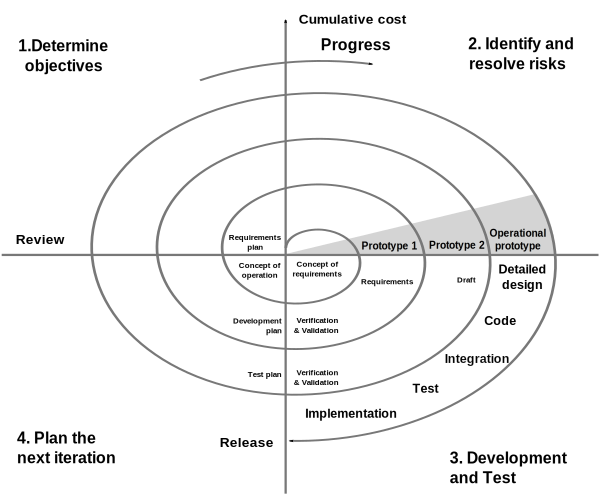
\includegraphics[width=0.8\textwidth]{spiral-model-softdevel}
  \end{center}
  \caption{the \textbf{traditional spiral development} model (from Wikipedia \href{https://en.wikipedia.org/wiki/Spiral_model}{spiral model})}
  \label{fig:tradspiral}
\end{figure}
%
But \RefPerSys' development follows a
\href{https://en.wikipedia.org/wiki/Strange_loop}{strange loop}
\cite{hofstadter:2007:strange-loop}, since it is bootstrapped in an
\href{https://en.wikipedia.org/wiki/Software\_prototyping\#Evolutionary\_prototyping}{evolutionary
  prototyping} manner. It is more like a spiral staircase like in
figure \ref{fig:bootstrap-stair}. The initial (floor) is just a
persistent system, and we gradually add new code implementing more
features (first entirely hand-written, later more and more parts of it
replaced by {\RefPerSys} generated code). Of course the fun is in
replacing existing hand-written code (or low-level DSL) by more
expressive and generated one. So we will continuously rewrite past
formalizations as a more clever and expressive ones, taking more and
more advantage of {\RefPerSys} whole-system introspective abilities.
All of \href{https://en.wikipedia.org/wiki/Eurisko}{\textsc{Eurisko}}
\cite{Lenat:1983:Eurisko},
\href{https://en.wikipedia.org/wiki/Cyc}{\textsc{Cyc}}
\cite{Lenat:1991:ev-cycl} and
\href{https://en.wikipedia.org/wiki/Self\_(programming_language)}{\textsc{Self}}\footnote{\textsc{Self}
was even able (in hours of CPU time) to redefines its integers -even
for arithmetic used inside its compiler- as
\href{https://en.wikipedia.org/wiki/Arbitrary-precision_arithmetic}{bignums}.}
\cite{chambers:1991:efficient} (or even
\href{https://iolanguage.org/}{\textsc{Io}} or
\href{https://en.wikipedia.org/wiki/Smalltalk}{\textsc{Smalltalk}})
systems and their incremental development process are inspirational.

\begin{figure}[h]
  \begin{center}
    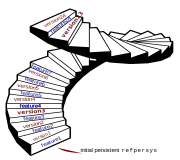
\includegraphics[width=0.8\textwidth]{spiral-stairs}
  \end{center}

  \begin{quote}
    \begin{relsize}{-0.2}
    Each new feature -or small incremental change or a few of them
    (small \texttt{git commit}s) - of {\RefPerSys} enables us to build
    and \textbf{generate} the next version of {\RefPerSys}, and a next
    feature is then added to that \textit{improved} version, and so on
    repeatedly, etc....
    \end{relsize}
  \end{quote}
  
  \caption{the strange \textbf{{\RefPerSys} staircase development model} {\relsize{-1}{(from a \href{https://thenounproject.com/term/spiral-stairs/956427/}{figure of Spiral stairs} by Lluisa Iborra from the Noun Project)}}}
  \label{fig:bootstrap-stair}
\end{figure}

The first significant milestone of {\RefPerSys} should be the ability
to re-generate all its textual source files (and maybe even
\texttt{git add} then\texttt{git commit} them). That would require
first implementing some simple template based
machinery\footnote{Perhaps inspired by simple designs like
  \href{https://docs.djangoproject.com/en/2.2/topics/templates/}{\textsc{Django}
    tempates}, but driven by frame-based {\RefPerSys} objects.}, withe
the ability, like
\href{https://en.wikipedia.org/wiki/Quine\_(computing)}{\textsc{Quine}}
programs do, to regenerate all {\RefPerSys} source code (e.g. in C++,
a \texttt{Makefile}, etc...). Actually {\RefPerSys} needs to
conceptually have \textbf{self-modifying code}
\cite{Tschudin:2005:HarnessingSC}, practically implemented by
systematically doing most function calls through indirect function
pointers (which gets updated with
\href{http://man7.org/linux/man-pages/man3/dlsym.3.html}{\texttt{dlsym(3)}}).

\bigskip

%%%%%%%%%%%%%%%%%%%%%%%%%%%%%%%%%%%%%%%%%%%%%%%%
\subsection{\textsc{RefPerSys} persistent heap}
\label{subsec:persistheap}

When {\RefPerSys} is running in some multi-threaded \textsc{Linux}
\href{https://en.wikipedia.org/wiki/Process\_(computing)}{process},
the {\RefPerSys} persistent heap is (like Bismon's one
\cite{Starynkevitch:2019:bismon-draft}) semantically like the memory
heap of most
\href{https://en.wikipedia.org/wiki/Dynamic\_programming\_language}{dynamic
  programming languages} (such as
\href{https://python.org/}{\textsc{Python}},
\href{https://www.gnu.org/software/guile/}{\textsc{Guile}},
\href{https://golang.org/}{\textsc{Go}},
\href{http://sbcl.org/}{\textsc{Sbcl}}, etc \ldots). The
%%\textcolor{red}{\textbf{\relsize{+1}{still incomplete}}}
figure \ref{fig:persistent-heap} should give an intuition about that
heap, when it is inside the
\href{https://en.wikipedia.org/wiki/Virtual_address_space}{virtual
  address space} of some \texttt{refpersys} process. We strongly want
to avoid any
\href{https://en.wikipedia.org/wiki/Global\_interpreter\_lock}{GIL},
but multi-threaded precise efficient garbage collector implementations
are quite difficult to code. However, notice that the persistence
(dump as textual \texttt{git}-versioned disk files) of a heap uses
algorithms similar to those of copying garbage collectors
\cite{wilson:1992:uniprocessorgc, jones:2016:gchandbook}.

\begin{figure}[H]
  \begin{center}
    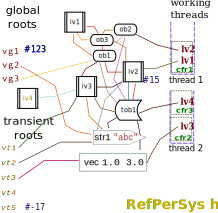
\includegraphics[width=0.8\textwidth]{heap-refpersys}
  \end{center}

\begin{quote}
  \begin{relsize}{-0.2}
    \begin{tabular}{ll}
      \texttt{\textbf{\textit{\#123}}} & a tagged 63 bits integer \\
      \texttt{\textit{vg1}} & a global persisted variable \\
      \texttt{\textit{vt2}} & a static transient variable \\
      \texttt{\textbf{ob1}} & a mutable persistent object \\
      \texttt{\textbf{iv2}} & an immutable constant composite value \\
      \texttt{\textbf{iv4}} & an immutable but \textbf{dead} constant composite value (should be GC-ed) \\
      \texttt{\textbf{tob1}} & a transient mutable object \\
      \texttt{str1} & a constant \textsc{utf-8} string value \texttt{"abc"} \\
      \texttt{vec} & a constant vector of floats {$ [1.0; 3.0] $} \\
      \texttt{\textit{lv2}} & a local variable inside its call frame \\
      \textit{cfr1} &  a \textbf{call frame} (simplified) \\
      \textit{\textbf{thread1}} & a \textbf{working thread} and its call stack (simplified) \\
    \end{tabular}
    \medskip

    In real life, the heap may be quite large (gigabytes) and contain
    hundreds of global roots or transient roots, millions of objects
    (sometimes transient, often persistent) and many millions
    immutable values (some of them composite and containing values,
    other scalar and containing non-pointer data like strings or
    vectors of float do), and dozen of working threads, each having
    thousands of call frames with dozens of local variables each.
   \end{relsize}
\end{quote}
  
  \caption{the  \textbf{{\RefPerSys} persistent heap}  (simplified)}
  \label{fig:persistent-heap}
\end{figure}

That figure \ref{fig:persistent-heap} shows a few global and transient
roots (both being processed by the garbage collector), and several
threads each having its call stack (made of call frames) with local
variables in it. In that figure, if $\mu$ and $\mu'$ are two memory
zones or locations (like for an object such as \texttt{ob1}, or for an
immutable value \texttt{iv2}), there is an arrow $\mu \rightarrow
\mu'$ if some field $\phi$ of $\mu$ refers to $\mu'$, that is (in C
like notation) if \fbox{$\mu$\texttt{\textbf{->}}$\phi = \mu'$}. Different
arrow colors could mean different fields $\phi, \phi' \ldots$ etc
\ldots The heap is actually a large directed graph and may contain
cycles (e.g. $ ob1 \rightarrow iv1 \rightarrow ob3 \rightarrow ob2
\rightarrow ob3 $). Most values are immutable values (some of them
being composite, such as \texttt{iv1}). Some immutable values are
scalar (e.g. strings). Notice that \texttt{iv4} is a dead value,
unreachable from others; it should be later garbage collected.  Only
objects have a content which may change. Since {\RefPerSys} is
multi-threaded, the access inside every object should be thread-safe
and usually is protected by a
\href{https://en.wikipedia.org/wiki/Lock\_(computer\_science)}{\textit{mutex}}
(or \textit{read write lock}) which is part of that object\footnote{Or
by atomic pointers, probably the {\RefPerSys} class of an object is,
inside it, given by some C++ field with an
\href{https://en.cppreference.com/w/cpp/atomic/atomic}{\texttt{std::atomic}}
pointer type, for efficiency reasons.}.


Conceptually, {\RefPerSys}
\href{https://en.wikipedia.org/wiki/Tracing_garbage_collection}{tracing
  precise garbage collector} should traverse the graph of references
to {\RefPerSys} values, starting from global or transient roots and
local variables inside call frames of working threads. Each
{\RefPerSys} \textbf{value} \index{value} (immutable or object) is
represented by a machine word (aligned, 64 bits) which usually
contains a pointer, but sometimes some
\href{https://en.wikipedia.org/wiki/Tagged\_pointer}{tagged integer}.
Immutable values are often ``small'' (typically, less than a few dozens of words of memory, sometimes a lot more) but
objects are necessarily heavier since they contain some kind of
lock. \href{https://en.wikipedia.org/wiki/Closure\_(computer_programming)}{closures}
are immutable values, containing an object representing and giving
their function code (as a C function pointer inside that object), and
additional closed values. In practice our garbage collector processes
not only values (either immutable values or objects), but also
\textbf{quasi-values} \index{quasi-value}: these are a single memory
zone which is allocated using the garbage collector allocation
protocol, traversed by the GC when something points to it, appears
inside other values (in particular, as payload \index{payload} of objects), but by
convention should not be passed as a genuine value. So the figure
\ref{fig:persistent-heap} is a simplification.

Some values (or objects) are dead; in the figure
\ref{fig:persistent-heap}, the immutable value \texttt{iv4} is not
reachable from roots or local variables on the call stack of working
threads. So it is dead and should eventually be reclaimed by the
garbage collector.

\textbf{Values} -either immutable values or changeable objects- in
       {\RefPerSys} can be either \textbf{persistent} (dumped in
       textual state files\footnote{In the current implementation,
       {\RefPerSys} state files should appear under
       \texttt{persistore/} subdirectory, and the manifest file is
       \texttt{rps\_manifest.json} at the top directory.}, then
       reloaded at restart of \texttt{refpersys} process) or
       \textbf{transient} (that is, not dumped and not appearing in
       state files).

The \textbf{persistence} machinery - the dump - is conceptually simple
and could run in several threads: start from global roots and traverse
the memory graph but ignore transient objects and transient roots and
memoize previously seen persistent objects. Of course, objects should
not be persisted twice, and are referred by the \textbf{object id} or
\textbf{objid} in the state files produced by the dump. That
\textit{objid} \index{objid@\textit{objid}} is alphanumeric, randomly generated and so hopefully
globally unique -like {\relsize{-1}{\texttt{\_2om48kc3k5R02d3ktW}}}
for example- in our current implementation; exactly like
\href{https://en.wikipedia.org/wiki/Universally_unique_identifier}{\textsc{Uuid}s}
should be. Notice the conceptual similarity between {\RefPerSys} dump
algorithm and its tracing garbage collector: both are traversing the
graph of references inside the heap.

The global roots are objects. Use the C++ functions
\texttt{rps\_each\_root\_object} to iterate on them,
\texttt{rps\_add\_root\_object} to add one,
\texttt{rps\_remove\_root\_object} to remove one,
\texttt{rps\_is\_root\_object} to test if an object is a global root,
\texttt{rps\_set\_root\_objects} to get the set of all of them,
and\texttt{rps\_nb\_root\_objects} to get their number. Of course,
some global roots can be transient objects, but all of them are roots
for the garbage collector.

The initial loading machinery (recreating a suitable heap - and
rebuilding a graph of references inspired by figure
\ref{fig:persistent-heap}, without any transient stuff) from its
previous dumped state) is first creating empty all objects, then later
filling each of them. However, for efficiency, we may want to load the
heap in parallel, using several loader threads. This could be easy if,
after having created all objects as empty, and loaded plugins
(i.e. \texttt{dlopen}-ing many \texttt{*.so} files), {\RefPerSys}
processes each state file in a potentially different loading thread.

\bigskip

%%%%%%%%%%%%%%%%%%%%%%%%%%%%%%%%%%%%%%%%%%%%%%%%
\subsection{Agenda and multi-threading in \RefPerSys}
\label{subsec:agenda-thread}

Once {\RefPerSys} persistence is implemented and provides some
meta-programming facilities, we can define and use some agenda
machinery. The insight is that {\RefPerSys} is running several
\cite{barney:2010:pthreads, butenhof:1997:programming} \textbf{worker
  threads}\footnote{Concretely, this means
\href{http://man7.org/linux/man-pages/man7/pthreads.7.html}{\texttt{pthreads(7)}},
perhaps wrapped as
\href{https://en.cppreference.com/w/cpp/thread}{\textsc{C++11}
  threads},
\href{https://doc.qt.io/qt-5/thread-basics.html}{\textsc{Qt5}
  threads},
\href{https://developer.gnome.org/glib/stable/glib-Threads.html}{\textsc{Glib}
  threads}, etc ....}  known to its garbage collector (which might
also need its own managing and synchronizing thread, which will mostly
stay idle.). Our \textbf{agenda} \index{agenda} is the central
mechanism of {\RefPerSys} feeding these worker threads with some work
to do, using \textbf{tasklets} representing a small amount of work to
be done.

\medskip

Each worker thread is indefinitely looping like this:
\begin{enumerate}
\item it runs occasionally some housekeeping processing, notably
  garbage collection work. This is where garbage collection gets
  synchronized. Occasionally, some new tasklets could be
  ``auto-magically'' inserted in the agenda at this point\footnote{Or
  such tasklets could be very carefully added into the agenda from
  non-worker threads organized in a producer-consumer fashion -such as
  those started by \texttt{libonion}-, respecting our GC
  invariants. This is a delicate issue !}, e.g. to run some code when
  some input data is available on some
  \href{https://en.wikipedia.org/wiki/File_descriptor}{file
    descriptor} for a
  \href{http://man7.org/linux/man-pages/man7/pipe.7.html}{\texttt{pipe(7)}}
  or a
  \href{http://man7.org/linux/man-pages/man7/tcp.7.html}{\texttt{tcp(7)}}
  socket, or to run some code every tenth of second, or to handle
  graceful termination when getting a \texttt{SIGTERM}\footnote{Read
  also
  \href{http://man7.org/linux/man-pages/man7/signal-safety.7.html}{\texttt{signal-safety(7)}}
  and consider using
  \href{http://man7.org/linux/man-pages/man2/signalfd.2.html}{\texttt{signalfd(2)}}
  or pipe-to-self tricks inspired by
  \href{https://doc.qt.io/qt-5/unix-signals.html}{\textsc{Qt} approach
    to \textsc{Unix} signal handling}. Notice that
  \href{http://man7.org/linux/man-pages/man2/timerfd\_create.2.html}{\texttt{timerfd\_create(2)}}
  might also be useful for tasklets to be added periodically in some
  \href{https://en.wikipedia.org/wiki/Event_loop}{event loop} around
  \href{http://man7.org/linux/man-pages/man2/poll.2.html}{\texttt{poll(2)}}.}
  \href{http://man7.org/linux/man-pages/man7/signal.7.html}{\texttt{signal(7)}}.
\item it waits, if so needed (probably using \textsc{Pthreads}
  condition variables), for the agenda to become non-empty
\item it chooses a tasklet $\tau$ to run inside the agenda. That
  tasklet is taken, so removed from the agenda.
\item it runs that tasklet $\tau$ for a small amount of time (a few
  dozen of milliseconds, typically), called a
  \textbf{step}\footnote{Calling blocking system calls such as
  \href{http://man7.org/linux/man-pages/man2/poll.2.html}{\texttt{poll(2)}}
  or
  \href{http://man7.org/linux/man-pages/man2/read.2.html}{\texttt{read(2)}}
  from a pipe or socket should be forbidden here, because a step
  should run quickly, in milliseconds.}. Of course during that step
  the agenda can (and usually will) change, and perhaps the same
  tasklet $\tau$ would be added again into the agenda, with maybe
  several other tasklets. Or on the contrary, running $\tau$ could
  remove one or several other tasklets $\tau_1, \tau_2 \ldots$ from
  the agenda, and add other ones $\tau'_1, \tau'_2, \ldots$ there.
\item that loop is repeated (unless {\RefPerSys} is stopped).
\end{enumerate}

The number of worker threads is fixed and small. Typically one worker
thread per processor core (so 3 on a small laptop, 20 or 30 on a big
desktop). Of course the agenda mechanism requires synchronization through
locks or mutexes and \textsc{Pthread} condition variables
\cite{barney:2010:pthreads}.

In addition of the worker thread, some additional slave threads could
be needed, in particular to handle some event loop (and serve HTTP
requests).  Of course the running steps should appropriately lock
objects, to avoid aftermath and synchronize properly their mutation.


The concrete organization of the {\RefPerSys} agenda has to be
precisely defined. It could be, as
\href{http://github.com/bstarynk/bismon}{\textsc{Bismon}} has, a small
data structure made of several first-in first-out queues, e.g. a queue
of high priority tasklets, another of medium priority tasklets, one of
low priority tasklets, etc..., with the agenda mechanism choosing in
the non-empty queue of highest priority its tasklet staying in front.

\bigskip

%%%%%%%%%%%%%%%%%%%%%%%%%%%%%%%%%%%%%%%%%%%%%%%%
\subsection{Metaprogramming and introspection in \RefPerSys}
\label{subsec:metaprog-introspec}

\textbf{Metaprogramming} \index{metaprogramming} is defined
\href{https://en.wikipedia.org/wiki/Metaprogramming}{in Wikipedia} as
``a programming technique in which computer programs have the ability
to treat other programs as their data. It means that a program can be
designed to read, generate, analyze or transform other programs, and
even modify itself while running''. That design idea is central to
many Artificial Intelligence systems and AI inspired
languages\footnote{See also \href{http://s48.org}{\textsc{Scheme 48}},
\href{http://sbcl.org/}{\textsc{SBCL}},
\href{http://https://www.rust-lang.org/}{\textsc{Rust}}, even
\href{https://en.cppreference.com/w/cpp/language/templates}{C++
  \emph{templates}}, \href{https://www.call-cc.org/}{\textsc{Chicken
    Scheme}}, \href{
  http://okmij.org/ftp/ML/MetaOCaml.html}{\textsc{MetaOCaml}}, the
\href{http://eclipseclp.org/}{\textsc{ECLiPSe} Constraint Programming
  System}, \href{https://www.rascal-mpl.org/}{\textsc{Rascal}},
\href{http://nemerle.org/}{\textsc{Nemerle}},
\href{http://coccinelle.lip6.fr/}{\textsc{Coccinelle}},
\href{{https://ocsigen.org/}}{\textsc{Ocsigen}},
\href{http://www.gprolog.org/}{\textsc{Gnu Prolog}},
\href{http://www.clipsrules.net/}{\textsc{Clips}},
\href{https://logological.org/gpp}{\textsc{Gpp}},
\href{http://swig.org/}{\textsc{Swig}},
\href{https://www.antlr.org/}{\textsc{Antlr}},
\href{https://github.com/drh/iburg}{\textsc{Iburg}},
\href{https://www.gnu.org/software/bison/}{Gnu \textsc{Bison}}, etc
\ldots} and is also common in software engineering\footnote{A typical
example is the \href{http://gcc.gnu.org}{\textsc{GCC}} compiler, or
\href{https://en.wikipedia.org/wiki/Autoconf}{\textsc{Autoconf}}, and
\href{https://en.wikipedia.org/wiki/Source-to-source_compiler}{transpiler
  approaches}} \cite{Lenat:1983:Eurisko, Lenat:1983:theory,
  Lenat:1991:ev-cycl, Pitrat:1996:FGCS, Pitrat:2009:AST,
  Pitrat:2009:ArtifBeings, Pitrat:blog, Queinnec:1996:LSP,
  Queinnec:2004:ContinWeb, Starynkevitch-1990-EUM,
  Starynkevitch-DSL2011, Starynkevitch-GCCMELTweb,
  Starynkevitch:2007:Multistage, Starynkevitch:2019:bismon-draft,
  Tschudin:2005:HarnessingSC, abelson:1996:sicp, briot:1987:uniform,
  chambers:1991:efficient, cointe:1987:metaclasses, dormoy:1992:meta,
  fouet-starynkevitch:describing-control:1987,
  greiner:1980:representation,
  hernandez-phillips:2019:debugging-bootstrap,hofstadter:2007:strange-loop,
  kay:1996:early-smalltalk, kelsey:1998:r5rs,
  kumar:2015:importance-expert-systems, matthews:2005:operational,
  mazur:2004:compile, nigro:2008:meta, queinnec:2003:lisp,
  Starynkevitch:2009:grow, serrano:1995:bigloo}.  Generating some
``source'' code at build time is usual practice, advocated also by the
\href{https://ninja-build.org/}{\textsc{Ninja} build system}, and
theorized (around 1930, before even computers existed) in the
\href{https://en.wikipedia.org/wiki/Church-Turing_thesis}{\textsc{Church-Turing}
  thesis}. Related concepts include the famous (but
\href{https://en.wikipedia.org/wiki/Undecidable_problem}{undecidable})
\href{https://en.wikipedia.org/wiki/Halting_problem}{\textbf{halting
    problem}} (whose proof involves a metaprogramming approach
\cite{Hofstadter:1979:GEB}),
\href{https://en.wikipedia.org/wiki/Hygienic_macro}{hygienic macros},
and \href{https://en.wikipedia.org/wiki/Rice's_theorem}{Rice's
  theorem}.

Practically speaking \cite{abelson:1996:sicp}, metaprogramming is
easier achieved by explicitly representing (maybe incomplete) code
with
\href{https://en.wikipedia.org/wiki/Abstract_syntax_tree}{abstract
  syntax trees} \index{abstract syntax tree} \index{tree!abstract
  syntax} (or \index{AST} AST), maybe with some holes for
\href{https://en.wikipedia.org/wiki/Metavariable}{metavariables} for
their later
\href{https://en.wikipedia.org/wiki/Explicit_substitution}{explicit
  substitution}, in the spirit of
\href{https://docs.djangoproject.com/en/2.2/topics/templates/}{\textsc{Django}
  templates} or of
\href{https://lispcookbook.github.io/cl-cookbook/macros.html}{\textsc{Common
    Lisp} macros} or
\href{https://en.wikibooks.org/wiki/Scheme_Programming/Macros}{\textsc{Scheme}
  macros}. A practical way to implement such a template machinery for
generating C or C++ code is given by
\href{https://gcc.gnu.org/wiki/MELT tutorial}{\textsc{GCC MELT} code
  chunks} \cite{Starynkevitch-DSL2011, Starynkevitch-GCCMELTweb,
  Starynkevitch:2009:grow, Starynkevitch:2007:Multistage}, where a
piece of C (or C++) code with holes (or metavariables)
\texttt{\$hellochunk} and \texttt{\$msg} is given through the
``macro-string''
\verb!#{/*$hellochunk#_here*/ printf("hello %s\n", $msg);}#! ... \\
Later, such a macro-string or code chunk can be expanded by filling
the holes, that is expanding the metavariables (e.g.\texttt{\$msg})
appropriately. Such an expansion might be recursive, since some hole
filling (or metavariable replacement) could in turn trigger expansions
of other macro-strings. In practice, {\RefPerSys} will use similar
code chunks and macro-expansion to generate its C (or C++) code, and
some initial ad-hoc
\href{https://en.wikipedia.org/wiki/Integrated_development_environment}{integrated
  development environment} \index{integrated development environment}
(or \index{IDE} IDE) will have to be coded, handling passively some
persistent store. The expansion will be done through some scripting
language (or \emph{domain specific language}, a.k.a. DSL) which has to
be implemented inside our IDE.


Metaprogramming involves code generation (using
\href{https://en.wikipedia.org/wiki/Source-to-source_compiler}{source-to-source}
ahead-of-time and/or
\href{https://en.wikipedia.org/wiki/Just-in-time_compilation}{just-in-time}\footnote{Several
JIT compilation libraries exist, notably
\href{https://gcc.gnu.org/onlinedocs/jit/}{\texttt{libgccjit}}
provided inside recent \href{http://gcc.gnu.org}{\textsc{GCC}}
compilers.} compilation techniques \cite{Aho:2006:dragon-book}, and in
     {\RefPerSys} is useful for many tasks, such as generating the
     garbage collection support routines for scanning or forwarding,
     and the loading and dumping routines needed for persistence (in
     the spirit of
     \href{https://en.wikipedia.org/wiki/RPCGEN}{\textsc{RpcGen}},
     \href{http://swig.org/}{\textsc{Swig}} and other
     \href{https://en.wikipedia.org/wiki/Serialization}{serialization}
     frameworks).

 In \RefPerSys, metaprogramming is often and practically achieved
 (like in \cite{Starynkevitch-DSL2011,
   Starynkevitch:2019:bismon-draft, Pitrat:1996:FGCS,
   Pitrat:2009:ArtifBeings} and our
 \href{https://github.com/bstarynk/misc-basile/blob/master/manydl.c}{\texttt{manydl.c}}
 example program), by generating some C or C++ code in a temporary
 file\footnote{There are practical reasons to generate these temporary
 files outside of \texttt{/tmp/}, which gets cleaned at reboot.} like
 \texttt{/tmp/rpsgen123.c}, compiling that file
 \cite{drepper:2011:write-shared-lib} into a generated plugin
 \texttt{/tmp/rpsgen123.so} by running a process such as
        {\relsize{-1}{\texttt{gcc -fPIC -Wall -O -g -shared
              /tmp/rpsgen123.c -l\textit{something} -o
              /tmp/rpsgen123.so}}} and waiting for its successful
        completion, then
        \href{http://man7.org/linux/man-pages/man3/dlopen.3.html}{\texttt{dlopen(3)}}-ing
        that newly generated \texttt{/tmp/rpsgen123.so}, in a manner
        compatible with our garbage collection and agenda
        invariants. We might later care about carefully
        \href{http://man7.org/linux/man-pages/man3/dlclose.3.html}{\texttt{dlclose(3)}}-ing
        that generated plugin, but in practice we accept some limited
        virtual memory plugin leak, and we could just dump
        appropriately our persistent state by mentioning in some
        generated
        \href{https://en.wikipedia.org/wiki/Manifest_file}{Manifest
          file} those plugins which should be saved (as generated C
        code) with the state.
 
 
\medskip

\href{https://en.wikipedia.org/wiki/Reflection_(computer_programming)}{Reflection}
is ``the ability of a process to examine, introspect, and modify its
own structure and behavior'' and also, for
\href{https://en.wikipedia.org/wiki/Self-reflection}{self-reflection},
the capacity `` to exercise introspection and to attempt to learn more
about their fundamental nature and essence''. (Wikipedia). It is
advocated (in \cite{Pitrat:2009:ArtifBeings}) that a similar approach
is (painfully) achievable in AI systems, and it would need both clever
\href{https://en.wikipedia.org/wiki/Backtracking}{backtracking} and
\href{https://en.wikipedia.org/wiki/Stack_trace}{backtracing}
techniques.
 Libraries such as Ian Taylor's
 \href{https://github.com/ianlancetaylor/libbacktrace}{\texttt{libbacktrace}}
 (which wants most of the code to be compiled with
 \href{https://en.wikipedia.org/wiki/DWARF}{\textsc{Dwarf} debugging}
 information\footnote{In practice we should compile our or other C or
 C++ code with both \texttt{-O2 -g} passed while
 \href{https://gcc.gnu.org/onlinedocs/gcc/Invoking-GCC.html}{invoking}
 \texttt{GCC} or \texttt{g++}, and this is indeed possible and
 practically works well enough.}) are helpful.

 Our precise garbage collector (see \S \ref{sec:dataobjmodel} below
 and \cite{rafkind:2009:precise-gc}, or
 \href{http://starynkevitch.net/Basile/qishintro.html}{\textsc{Qish}})
 wants local variables holding garbage collected pointers to be known
 to the GC. In practice, the {\RefPerSys} call frame is some explicit
 local \texttt{struct} named \texttt{\_} in generated C
 code\footnote{Like \href{http://github.com/bstarynk/bismon/}{Bismon}
 does, see its \texttt{LOCAL\_BM} macro. See also the
 \texttt{CAMLparam$i$} and \texttt{CAMLlocal$j$} C macros of
 \href{https://caml.inria.fr/pub/docs/manual-ocaml/intfc.htm}{\textsc{OCaml}},
 and the \texttt{Py\_VISIT} and \texttt{Py\_DECREF} and other macros
 of
 \href{https://docs.python.org/3/extending/}{\textsc{Python}}, the \href{http://www.sbcl.org/manual/index.html\#Foreign-Function-Interface}{\textit{foreign function interface} of \textsc{SBCL}}, etc \ldots}. Such
 explicited local frames can often be optimized by \texttt{GCC} or
 \texttt{g++} (invoked with \texttt{-O2}).

 As suggested by Pitrat (see \cite{Pitrat:1996:FGCS, Pitrat:2009:AST,
   Pitrat:2009:ArtifBeings}), call stack reflection and backtrace is
 the elementary brick of more sophisticated \emph{introspection}
 techniques. At some point, our {\RefPerSys} system should inspect its
 call stack and may take decisions after that. A typical approach
 would be to run such introspection once in a while (e.g. every 0.1
 second on the average\footnote{Timing considerations are essential,
 practically speaking, in \RefPerSys. See
 \href{http://man7.org/linux/man-pages/man7/time.7.html}{\texttt{time(7)}}
 man page.}, in the
 \href{https://en.wikipedia.org/wiki/Inference_engine}{inference
   engine} of some
 \href{https://en.wikipedia.org/wiki/Expert\_system}{expert system} or
 \href{https://en.wikipedia.org/wiki/Knowledge_base}{knowledge base}
 component of {\RefPerSys}.

 \smallskip

 Since we aim to be able to re-generate most (and hopefully all) of
 {\RefPerSys} code (in C or in C++), having simple \textbf{coding
   conventions} does matter: every \RefPerSys-defined C or C++
 identifier should start with \texttt{rps\_} in lower, upper, or mixed
 case (e.g. also \texttt{RPS\_} or \texttt{Rps\_}). Every C or C++
 function, even \texttt{static inline} ones appearing in header files,
 has its name starting with \texttt{rps\_} and is \emph{globally}
 unique to the entire \texttt{refpersys} program. The C (or C++) code
 should be automatically indented\footnote{With the social convention
 that {\RefPerSys} contributors are running \texttt{omake indent} or
 \texttt{make indent} before every \texttt{git commit}!} using
 \href{https://www.gnu.org/software/indent/}{Gnu \textsc{Indent}} or
 \href{http://astyle.sourceforge.net/}{\textsc{Astyle}}. Every named
 \texttt{struct} (in C) should have its tag matching
 \texttt{rps\_*st}. Every \texttt{typedef}-ed data type should have
 its name matching \texttt{rps\_*t}. Every named \texttt{enum} should
 have its tag matching \texttt{rps\_*en} and the various enumerated
 values like \texttt{RPS\_*}. Even in cases the C (or the C++)
 language allows several name spaces\footnote{In C, having both a type
 and a label named \texttt{foo} is permitted, but we refuse such
 non-sense.}, we don't use that facility. Hence we refuse to code the
 common \texttt{typedef struct rpsfoo\_t rpsfoo\_t;} but prefer
 instead (inspired by \href{http://gtk.org}{\textsc{Gtk}}) coding
 \texttt{typedef struct rps\_\textit{foo}\_st
   rps\_\textit{foo}\_t}. Of course, names of
 \href{https://en.wikipedia.org/wiki/Local\_variable}{local variables}
 (that is
 \href{https://en.wikipedia.org/wiki/Automatic_variable}{automatic
   variables} with their
 \href{https://en.wikipedia.org/wiki/Scope\_(computer\_science)\#Lexical\_scoping}{lexical
   scope} limited to some small C or C++
 \href{https://en.wikipedia.org/wiki/Block\_(programming)}{block})
 could be as short as a single letter such as \texttt{i}. In general,
 our C or C++ code is written with the hope of being easily able to
 regenerate it.
 
\bigskip

%%%%%%%%%%%%%%%%%%%%%%%%%%%%%%%%%%%%%%%%%%%%%%%%%%%%%%%%%%%%%%%%
\section{The data and object models of \RefPerSys}
\label{sec:dataobjmodel}

The data is what is processed by {\RefPerSys}, and is made of values
(and, internally for the GC, also of quasi-values, which are pointers
to GC-managed memory zones). The object model is defining our classes,
our single inheritance mechanism, our message sending protocol (see \S
\ref{subsubsec:message-sending}).

%%%%%%%%%%%%%%%%%%%%%%%%%%%%%%%%%%%%%%%%%%%%%%%%
\subsection{how data should be processed in \RefPerSys}
\label{subsec:howdata}

{\RefPerSys} aiming to be first a good old fashioned AI system
(\href{http://bootstrappingartificialintelligence.fr/WordPress3/2013/12/the-future-of-ai-is-the-good-old-fashioned-artificial-intelligence/}{\textsc{Gofai}}),
better known as
\href{https://en.wikipedia.org/wiki/Symbolic\_artificial\_intelligence}{symbolic
  artificial intelligence} system, it is targetting mostly
\href{https://en.wikipedia.org/wiki/Computer\_algebra}{symbolic
  computation}, in particular using a
\href{https://en.wikipedia.org/wiki/Semantic\_network}{semantic
  network} or other forms of mathematical finite but large
\href{https://en.wikipedia.org/wiki/Graph\_(discrete\_mathematics)}{graph}
representations, in particular
\href{https://en.wikipedia.org/wiki/Abstract\_syntax\_tree}{abstract
  syntax trees}\footnote{Practically speaking, abstract syntax trees
are in fact at least finite
\href{https://en.wikipedia.org/wiki/Directed_acyclic_graph}{directed
  oriented graphs} and could even have cycles if you relate a
\href{https://en.wikipedia.org/wiki/Symbol\_(programming)}{symbol} to
its properties.} of generated programs, of internal rules or
expressions, by some internal metaprogramming machinery. So
{\RefPerSys}
\href{https://en.wikipedia.org/wiki/Object_(computer_science)}{objects}
should have a finite but changing set of
\href{https://en.wikipedia.org/wiki/Attribute_(computing)}{attributes}
or
\href{https://en.wikipedia.org/wiki/Property_(programming)}{properties}
and be organized, as in most
\href{https://en.wikipedia.org/wiki/Object-oriented_programming}{object-oriented
  languages}. Hence,
\href{https://en.wikipedia.org/wiki/Electronic\_document}{documents},
\href{https://en.wikipedia.org/wiki/Hypertext}{hypertext}, high-level
\href{https://en.wikipedia.org/wiki/Source\_code}{source code},
\href{https://en.wikipedia.org/wiki/Ontology\_(information\_science)}{ontologies},
\href{https://en.wikipedia.org/wiki/Knowledge\_base}{knowledge bases},
\href{https://en.wikipedia.org/wiki/Expert\_system}{expert systems},
implementation of some
\href{https://en.wikipedia.org/wiki/Inference_engine}{inference
  engine} guided by
\href{https://en.wiktionary.org/wiki/metarule}{metarules}, etc \ldots~
should all be easily and conveniently representable\footnote{So
\href{https://en.wikipedia.org/wiki/Artifact_(software_development)}{artifacts}
like \href{https://en.wikipedia.org/wiki/XML}{\textsc{Xml}} documents,
\href{https://en.wikipedia.org/wiki/HTML5}{\textsc{Html5}} or
\href{https://en.wikipedia.org/wiki/XHTML}{\textsc{Xhtml}} hypertexts,
\href{http://json.org/}{\textsc{Json}} data,
\href{https://yaml.org/}{\textsc{Yaml}} representations should all be
easily representable and inspirational for {\RefPerSys} data and its
processing.}  and processable, as some evolving subgraph of
{\RefPerSys} values.

Since {\RefPerSys} objects are the only mutable values, they keep not
only their synchronization data, but also attributes or properties,
components, and some extra \index{payload}
\textbf{payload}\footnote{From the GC point of view, payloads are
quasi-values \index{quasi-value} \ldots}. See also \S
  \ref{subsec:mutable-objects} below.

The {\RefPerSys} worker threads, organized in a small
\href{https://en.wikipedia.org/wiki/Thread_pool}{thread
  pool}\footnote{Threads are heavy resources, each of them needing a
call stack and, practically speaking, a processor core to run. We
surely want to have at most a dozen of worker threads.} are somehow
organized in some
\href{https://en.wikipedia.org/wiki/Agenda}{\textbf{agenda}}\footnote{In
Latin, ``agenda'' means ``things which have to be done or
completed''.}  mechanism. Informally, the agenda is a clever
organization (perhaps a few mostly
\href{https://en.wikipedia.org/wiki/FIFO}{FIFO}
\href{https://en.wikipedia.org/wiki/Queue\_(abstract\_data\_type)}{queue}
of elementary tasklets, or something more complex). Each such tasklet
runs for a short time\footnote{In practice, several dozens of
milliseconds, to play nice with human interaction and be friendly with
our garbage collector} and may, while running, update that agenda by
adding further runnable tasklets to it, or by removing some of
them. The agenda itself should be somehow reified and partly
persistent, and tasklets are {\RefPerSys} objects. Of course some
tasklets (e.g. those directly related to the user interface,
e.g. \href{https://en.wikipedia.org/wiki/Ajax_(programming)}{\textsc{Ajax}}
or \href{http://qt.io/}{\textsc{Qt}} callbacks) are transient.

%%%%%%%%%%%%%%%%%%%%%%%%%%%%%%%%%%%%%%%%%%%%%%%%
\label{subsec:datalowhigh}
\subsection{data at the low and high levels}

{\RefPerSys} mostly handle values\footnote{In particular, only
\textsc{closures} are
\href{https://en.wikipedia.org/wiki/Function_application}{applied}, to
arguments which are values (read more about
\href{https://en.wikipedia.org/wiki/Lambda_calculus}{$\lambda$-calculus});
or messages are sent, to values with perhaps additional value
arguments. Internally, our GC also handle quasi-values.}, which can be
either ``light'' immutable values or ``heavy'' mutable objects. Our
data model is inspired by the
\href{https://en.wikipedia.org/wiki/ObjVlisp}{\textsc{ObjVLisp}} model
(or
\href{https://en.wikipedia.org/wiki/Common_Lisp_Object_System}{\textsc{CLOS}},
see also the
\href{http://www.lispworks.com/documentation/HyperSpec/Front/index.htm}{Common
  Lisp HyperSpec}) common in most Lisp implementations
\cite{queinnec:2003:lisp, cointe:1987:metaclasses, briot:1987:uniform}
and inspired by
\href{https://en.wikipedia.org/wiki/Smalltalk}{\textsc{Smalltalk}}
\cite{kay:1996:early-smalltalk}. Also, a value can be transient or
persistent. Each {\RefPerSys} value fits in one 64 bits machine
word\footnote{Remember: {\RefPerSys} targets only Linux x86-64
systems!}, so is nicely represented as an aligned pointer (ending with
a 0 bit) or a tagged integer (63 bits, with the least significant bit
being set to 1). Values are usually pointers to complex structures,
so, per the
\href{https://github.com/hjl-tools/x86-psABI/wiki/x86-64-psABI-1.0.pdf}{x86-64
  calling conventions}, are word aligned (address multiple of 8
bytes). Let's call \emph{genuine values} \index{genuine!value} those
that are not
\href{https://medium.com/@hinchman_amanda/null-pointer-references-the-billion-dollar-mistake-1e616534d485}{\texttt{null}}
and not tagged pointers (so either immutable values or objects in
figure \ref{fig:persistent-heap}). These \textbf{genuine values} (and
also quasi-values) are practically implemented as a \href{
  https://en.wikipedia.org/wiki/Tagged_union}{tagged
  union}\footnote{An old example of tagged unions in C is the
\href{https://tronche.com/gui/x/xlib/events/structures.html}{X11 event
  structure}, but
\href{https://www.gnu.org/software/guile/manual/html\_node/A-Simple-Representation.html}{\textsc{Guile}}
and
\href{https://caml.inria.fr/pub/docs/manual-ocaml/intfc.html}{\textsc{OCaml}}
use similar implementation tricks.} and each of them start with a
field (probably 16 bits) identifying their concrete type.


\medskip

\subsubsection{values and quasi-values}
\label{subsubsec:values-quasi}

The {\RefPerSys} garbage collector manages both values and
quasi-values (that is, a single non-empty sequence of memory words,
used for some garbage collected data, e.g. inside objects). But only
persistent values are dumped and reloaded in the persistent store.
The values which are not dumped -so not reloaded on the next run- are
called \emph{transient} values.

  For pragmatical reasons, our values\footnote{Of course, quasi-values
  need not to be ordered and hashed!} should be both ordered and
  hashed, since many
  \href{https://en.wikipedia.org/wiki/Data\_structure}{data
    structures} \cite{cormen:2009:introduction}, specified as some
  \href{https://en.wikipedia.org/wiki/Abstract_data_type}{abstract
    data type}, either uses some ordering
  (e.g. in \href{https://en.wikipedia.org/wiki/Red-black_tree}{red-black
    trees}) or some hash-code (e.g. various kinds of
  \href{https://en.wikipedia.org/wiki/Hash_table}{hash
    tables}). Because of the weird and counter-intuitive semantics of
  \href{http://floating-point-gui.de}{floating point} numbers, the
  \href{https://en.wikipedia.org/wiki/NaN}{\textsc{NaN}} should be
  handled specifically (it is unordered), if we
  \href{https://en.wikipedia.org/wiki/Object\_type\_(object-oriented\_programming)\#Boxing}{box}
  IEEE \texttt{double}s.


  
  \medskip

\subsubsection{implementation details}
\label{subsubsec:implementation-details}

{\RefPerSys} takes advantage of some practical features\footnote{We
don't really care if these features are not exactly standard C11
\cite{c11-standard:2011}, because we strongly believe they are present
on practical Linux x86-64 computers.} of C on Linux x86-64:

\begin{itemize}
  \item Practically, machine data pointers should be at least 64 bits
    (8 bytes) aligned\footnote{The
  \href{https://en.wikipedia.org/wiki/X86-64}{\textsc{x86-64}} or
  \textsc{amd64}
  \href{https://en.wikipedia.org/wiki/Instruction_set_architecture}{instruction
    set architecture} allows in principle unaligned memory accesses,
  but these are very slow and unfriendly to
  \href{https://en.wikipedia.org/wiki/Cache_coherence}{cache
    coherence} hardware implementations.} for large enough memory
    zones (i.e. most practical \texttt{struct}-s), annd preferably 128
    bits, that is 16 bytes, aligned. See also the
    \href{https://en.cppreference.com/w/c/language/_Alignof}{\texttt{alignof}}
    macro of \texttt{<stdalign.h>} and the
    \href{https://gcc.gnu.org/onlinedocs/gcc/Common-Type-Attributes.html}{\texttt{aligned}
      type attribute}.
    
  \item Limited
    \href{https://en.wikipedia.org/wiki/Type_punning}{type-punning}
    abilities. {\relsize{-0.5}{Assume we have two \texttt{struct}-ures
        definitions, so \texttt{struct s1} and \texttt{struct
          s2}. Assume that both \texttt{s1} and \texttt{s2}
        \emph{start} with the same \emph{common} fields
        \texttt{unsigned num;} then \texttt{void*ptr;} followed by
        \texttt{char str[24];}. Assume that a pointer \texttt{p}
        points to a valid memory zone, whose alignment (respectively
        size) are at least all of \texttt{alignof(struct s1)},
        \texttt{sizeof(struct s1)}, \texttt{alignof(struct s2)},
        \texttt{sizeof(struct s2)}: so we have
        \texttt{alignof(typeof(*p)) >= alignof(struct s1) \&\&
          sizeof(*p) >= sizeof(struct s1)} and
        \texttt{alignof(typeof(*p)) >= alignof(struct s2) \&\&
          sizeof(*p) >= sizeof(struct s2)}. Then: \texttt{((struct
          s1*)p)->num} and \texttt{((struct s2*)p)->num} both refer to
        the same memory location and number there; \texttt{((struct
          s1*)p)->ptr} and \texttt{((struct s2*)p)->ptr} both refer to
        the same memory location and pointer there; and of course
        \texttt{((struct s1*)p)->str} and \texttt{((struct
          s2*)p)->str} is the \emph{same} string.}} See also
    \texttt{may\_alias}, \texttt{warn\_if\_not\_aligned},
    \texttt{aligned}, \texttt{transparent\_union} \textsc{GCC}
    \href{https://gcc.gnu.org/onlinedocs/gcc/Common-Type-Attributes.html}{type
      attributes}, the
    \href{https://gcc.gnu.org/onlinedocs/gcc/C-Dialect-Options.html}{\texttt{-fms-extensions}
      option} to \texttt{GCC}, and its
    \href{https://gcc.gnu.org/onlinedocs/gcc/Unnamed-Fields.html}{unnamed
      fields} ability.

    \item \href{https://en.wikipedia.org/wiki/Tail_call}{Tail call}
      optimization, practically provided in \emph{some} common cases
      by recent \href{http://gcc.gnu.org/}{\textsc{GCC}} or
      \href{http://clang.llvm.org/}{\textsc{Clang/LLVM}} compilers
      (requiring probably \texttt{-O2} compiler flag).

      \item Common
        \href{https://gcc.gnu.org/onlinedocs/gcc/C-Extensions.html}{extensions
          to the C language}, notably
        \href{https://gcc.gnu.org/onlinedocs/gcc/Statement-Exprs.html}{statement
          exprs} (very useful),
        \href{https://gcc.gnu.org/onlinedocs/gcc/Labels-as-Values.html}{label
          as values} (or ``computed \texttt{goto}''-s),
        \href{https://gcc.gnu.org/onlinedocs/gcc/Typeof.html#Typeof}{\texttt{typeof}},
        \href{https://gcc.gnu.org/onlinedocs/gcc/Zero-Length.html}{zero-length}
        arrays and
        \href{https://en.wikipedia.org/wiki/Flexible\_array\_member}{flexible
          array members},
        \href{https://gcc.gnu.org/onlinedocs/gcc/Return-Address.html}{return
          addresses} and
        \href{https://gcc.gnu.org/onlinedocs/gcc/Other-Builtins.html}{other
          built-ins}, may be used in {\RefPerSys} code.
\end{itemize}

\smallskip

Practically speaking, every {\RefPerSys} value or quasi-value (see our
\texttt{Rps\_QuasiZone} class) which sits in memory\footnote{This
excludes tagged integers, and that memory zone is at least word
aligned to 8 bytes.} is represented in some \texttt{class} inherited
from \texttt{Rps\_ZoneValue} For instance, our string values have
their memory zone type declared as \texttt{Rps\_String}, but we use
the \texttt{Rps\_StringValue} class to construct them. In
\texttt{Rps\_String} the field \texttt{\_sbuf} is a
\href{https://en.wikipedia.org/wiki/Flexible_array_member}{flexible
  array member}, and by convention contains \texttt{\_bytsiz + 1}
bytes (terminated with a 0 byte), is validly \textsc{Utf-8} encoded,
aligned to 4 bytes and nul-byte terminated. Hash codes cannot be 0 and
are lazily computed (so the \texttt{rps\_strhash} field is computed
once when it was 0). The \texttt{Rps\_Type::String} is some enumerator
inside a global \texttt{enum}. Strings are ordered naturally, using
\texttt{strcmp} on their \texttt{rps\_strdata} bytes.


\smallskip

The \texttt{refpersys} executable is handling files either from the
{\RefPerSys} home directory (obtained inside C++ code using
a \texttt{rps\_homedir()} call), given by \texttt{\$REFPERSYS\_HOME} or
\texttt{\$HOME} environment variables or thru the
\texttt{-{-}refpersys-home} program argument, or from the {\RefPerSys}
load directory (by default the source directory, or given thru the
\texttt{-{-}load} program argument). User preferences should go into the
       {\RefPerSys} home directory, e.g. as the
       \texttt{.refpersys.json} file there.

\textcolor{red}{@@TODO: should explain more implementation details in C++ terms?}


\medskip

%%%%%%%%%%%%%%%%%%%%%%%%%%%%%%%%%%%%%%%%%%%%%%%%
\subsection{immutable values}
\label{subsec:immutable-values}

By definition, immutable values don't change. All their useful
bits\footnote{For housekeeping purposes, our garbage collector may
reserve a few bits, e.g. for
\href{https://www.memorymanagement.org/glossary/t.html}{tri-color}
marking \cite{wilson:1992:uniprocessorgc}} stay unchanged as long as
the value is alive. Some values are scalar (strings, vectors of
floats, perhaps bitmaps\footnote{In practice, bitmaps or pixmaps would
rather be the payload of some objects, see below.} if we reify
them). Other values are composite.

Since objects are fundamental, we want to keep finite collections of
them. In particular, {\RefPerSys} will reify (represent as first-class
\emph{immutable} values)
\href{https://en.wikipedia.org/wiki/Tuple}{\textbf{tuples}}
\index{tuple} of objects and finite
\href{https://en.wikipedia.org/wiki/Set_(abstract_data_type)}{\textbf{sets}}
of objects as values, and also , and they are the common composite
values of \RefPerSys. A tuple is obviously represented by boxing a
sequence of object references (i.e. pointers). A set would be
represented by an ordered sequence of object pointers, with membership
efficiently testable by a
\href{https://en.wikipedia.org/wiki/Time\_complexity}{$O(log~ n)$}
time
\href{https://en.wikipedia.org/wiki/Binary_search_algorithm}{binary
  search algorithm}). We expect most of tuples and sets to be small
and fitting in an
\href{https://en.wikipedia.org/wiki/Cache\_hierarchy}{L1 or L2 cache
  line}, so their processing should be efficient.

In {\RefPerSys},
\href{https://en.wikipedia.org/wiki/Closure_(computer_programming)}{closures}
-that is first-class procedural values, like in
\textsc{Scheme}\footnote{Try for example \textsc{Gnu}
  \href{https://www.gnu.org/software/guile/}{\textsc{Guile}} following
  \href{http://starynkevitch.net/Basile/guile-tutorial-1.html}{this
    tutorial}.} \cite{kelsey:1998:r5rs, matthews:2005:operational,
  Queinnec:1996:LSP, Queinnec:2004:ContinWeb, abelson:1996:sicp},
\href{http://hop.inria.fr/home/index.html}{\textsc{Hop}} or
\href{https://www-sop.inria.fr/mimosa/fp/Bigloo/}{\textsc{Bigloo}}
\cite{serrano:1995:bigloo},
\href{http://www.lispworks.com/documentation/HyperSpec/Front/index.htm}{\textsc{Common
    Lisp}},
\href{https://en.wikipedia.org/wiki/JavaScript}{\textsc{JavaScript}} -
are also immutable values. The closed values -binding free variables
of the closure- inside such closures are arbitrary, but fixed, and
won't change during the lifetime of that closure. The function code
inside them is given by some fixed object reifying that code, and
probably useful to generate the ``source'' code (e.g. as generated
\emph{C} or \emph{C++} code) of that function. The
\href{https://en.wikipedia.org/wiki/Name_mangling}{mangled name},
later
``\href{http://man7.org/linux/man-pages/man3/dlsym.3.html}{\texttt{dlsym(3)}}-ed'',
of that function in its
\href{https://en.wikipedia.org/wiki/Executable_and_Linkable_Format}{ELF}
\texttt{*.so}
\href{https://en.wikipedia.org/wiki/Library\_(computing)\#Shared\_libraries}{shared
  object} file \cite{drepper:2011:write-shared-lib,
  levine:1999:linkers-loaders} is somehow related\footnote{For a
  fictional example, an object of objid \texttt{\_6lNdgIkKhwD04laO94}
  might be related to some ELF function of name close to
  \texttt{rps\_6lNdgIkKhwD04laO94}, etc \ldots} to the \emph{objid} of
that object. Closures are absolutely essential in {\RefPerSys}, since
they are the only way to refer to executable machine code. Even method
implementations are using closures, since the
\href{https://en.wikipedia.org/wiki/Virtual_method_table}{virtual
  method table} in {\RefPerSys} classes (actually, their payload) is
referring to closures (is is an association between selectors (like in
\href{https://en.wikipedia.org/wiki/Objective-C\#Messages}{Objective-C},
but reified as objects) and closures implementing methods, à la
\textsc{ObjVLisp} \cite{cointe:1987:metaclasses,
  abadi:1995:imperative}).

We may consider also having in {\RefPerSys} immutable
node\footnote{\RefPerSys nodes are generalizing \textsc{Bismon} nodes
\cite{Starynkevitch:2019:bismon-draft}, which are immutable, have an
object connective and a sequence of sons which are arbitrary
values. Perhaps ``node'' is a wrong word and we could name them
``records'' or ``structures''.}  instances: like mutable objects (see \S
\ref{subsec:mutable-objects} below), each of them would have a class
(with single-inheritance), attributes and components. But since they
are immutable, they have no objid, no locking mechanism, and their
class, attributes and components would be fixed and defined at their
creation time.

In C++ code, values are \texttt{Rps\_Value}, a ``smart'' value
container, actually a single word. That class is specialized into
helper subclasses, such as \texttt{Rps\_StringValue},
\texttt{Rps\_DoubleValue} etc.

\subsubsection{immutable scalar values}
\label{subsubsec:immutable-scalar}

Immutable scalar values include:
\begin{itemize}
  \item \textbf{strings}, \index{string} persisted as \textsc{Json} strings; their internal
    representation is \texttt{Rps\_String} using an \textsc{Utf-8}
    encoding. In C++, use \texttt{Rps\_String::make} to make one, or
    construct an \texttt{Rps\_StringValue} with a C or C++ \textsc{Utf-8} encoded
    string, a \texttt{std::string}, or a \texttt{QString}.
    \item boxed \textbf{doubles}\footnote{See
    \href{http://floating-point-gui.de}{\texttt{floating-point-gui.de}}
      for more about
      \href{https://en.wikipedia.org/wiki/IEEE\_754}{\textsc{Ieee 754}
        double precision numbers} on current computers. This is
      actually a difficult topic.} (which cannot hold an
    \textsc{Ieee-754} \texttt{NaN}, which is incomparable), persisted
    as \textsc{Json} doubles; their internal boxed representation is
    \texttt{Rps\_Double}. In C++, use \texttt{Rps\_Double::make} to make one, or
    construct an \texttt{Rps\_DoubleValue} with a C \texttt{double}.
\end{itemize}

\subsubsection{immutable composite values}
\label{subsubsec:immutable-composite}

Immutable composite values include:
\begin{itemize}
\item \textbf{tuples} of object references. Their memory
  representation is a \texttt{Rps\_TupleOb} zone, and it has both
  \texttt{Rps\_TupleOb::make} and \texttt{Rps\_TupleOb::collect} static functions. But use
  \texttt{Rps\_TupleValue} to build them. \textcolor{red}{@@TODO:
    should explain more}
\item \textbf{set} of object references; Their memory
  representation is a \texttt{Rps\_SetOb} zone, and it has both
  \texttt{Rps\_SetOb::make} and \texttt{Rps\_SetOb::collect} static functions. But use
  \texttt{Rps\_SetValue} to build them.  \textcolor{red}{@@TODO: should explain more}
\end{itemize}
\textcolor{red}{@@TODO: should explain a lot more}

%%%%%%%%%%%%%%%%%%%%%%%%%%%%%%%%%%%%%%%%%%%%%%%%%%%%%%%%%%%%%%%%
\subsection{mutable objects}
\label{subsec:mutable-objects}

Practically speaking, mutable objects are heavy, since they should
carry inside them locking devices\footnote{At the implementation
level, think of some
\href{https://computing.llnl.gov/tutorials/pthreads/\#Mutexes}{mutex}
or preferably some
\href{http://tuxthink.blogspot.com/2013/02/using-read-write-lock-in-pthreads.html}{read-write
  lock, so
  \href{https://pubs.opengroup.org/onlinepubs/7908799/xsh/pthread\_mutex\_init.html}{\texttt{pthread\_mutex\_init}}
  or
  \href{https://pubs.opengroup.org/onlinepubs/7908799/xsh/pthread_rwlock_init.html}{\texttt{pthread\_rwlock\_init}}}
or \href{https://en.cppreference.com/w/cpp/thread}{C++11
  equivalents}.} for multi-threading support. And each object carries
an association between attributes (playing the role of arbitrary keys)
and their corresponding value. In addition, an object can carry its
payload\footnote{Every payload belongs to a single object, its owner!}
for stuff which does not fit into that model. For example, an object
may carry as its payload a dictionary associating machine strings to
values, or an hash-table of triplets, or an opened \texttt{FILE*}
handle, or \href{https://en.wikipedia.org/wiki/File\_descriptor}{file
  descriptor}\footnote{\href{https://en.wikipedia.org/wiki/Finalizer}{Finalizers}
are practically not enough to handle these, even if they are useful,
in our GC, as a last resort mesure!}, or some
\href{https://www.tensorflow.org/}{\textsc{TensorFlow}} or
\href{https://gudhi.inria.fr/}{\textsc{Ghudi}} data for machine
learning purposes, maybe something related to
\href{https://github.com/davidmoreno/onion/}{\texttt{libonion}} or
\href{http://zeromq.org}{\texttt{ZeroMQ}}, some
\href{https://gmplib.org/}{\textsc{GMPlib}} big number, some
\href{https://www.bugseng.com/ppl}{\texttt{PPL}} polyhedra, maybe some
\href{http://qt.io/}{\textsc{Qt}} graphical widget, etc \ldots. Of
course every object has its class (which is itself an object, having a
\href{https://en.wikipedia.org/wiki/Metaclass}{metaclass}) and carries
a function pointer\footnote{That function pointer should be, for
efficiency reasons (we don't want to lock an object to get that
pointer!)
\href{https://en.cppreference.com/w/c/atomic}{\texttt{atomic}} in C
parlance, and might be set using
\href{http://man7.org/linux/man-pages/man3/dlsym.3.html}{\texttt{dlsym(3)}}.}, for {\RefPerSys} closures.

Notice that a generational GC approach moving data is possible for
some immutable values, but not for objects and their optional payload,
since {\RefPerSys} objects contain locks and payloads that are dealt
with through external functions requiring fixed, unchangeable, pointers.

In C++ code, object references are \texttt{Rps\_ObjectRef}, a
``smart'' object container, actually a single word. They are persisted
by their \textit{objid} in \textsc{Json} format as a string.

\subsubsection{objects as frame-like data}
\label{subsubsec:obj-frame}

{\RefPerSys} objects are quite flexible, even more than
\textsc{JavaScript}\footnote{Remember that in \textsc{JavaScript}
\textbf{\texttt{ob.fl}} is defined to be the same as
\texttt{ob['fl']}, the equivalent of fetching attribute or field
\texttt{fl} from an object \texttt{ob}. And \textbf{\texttt{ob[1]}} is
like component of index 1 in object \texttt{ob}.} ones; they take some
inspiration from \textsc{Rll} \cite{greiner:1980:representation},
\textsc{Eurisko} \cite{Lenat:1983:Eurisko, Lenat:1983:theory},
\href{https://en.wikipedia.org/wiki/Cyc}{\textsc{Cyc}} and its
\textsc{Cycl} \cite{Lenat:1991:ev-cycl}, and more recently the
\href{https://en.wikipedia.org/wiki/Semantic_Web}{\textit{Semantic
    Web}} and its
\href{https://www.w3.org/TR/owl-ref/}{\textsc{Owl}}. An object has
attributes (usually a few ones, but perhaps many of them) and
components (again, perhaps 0 or a few of them, but in rares cases
thousands of them), and some optional payload (quite often, it is
missing). Notice the similarity with \textsc{JavaScript} objects
(which calls \emph{fields} with \emph{keys} what {\RefPerSys} calls
attributes, and array elements what are {\RefPerSys}
components). However, \textsc{JavaScript} is (like
\href{http://iolanguage.com/}{\textsc{Io}} or \textsc{Self}
\cite{chambers:1991:efficient}) a
\href{https://en.wikipedia.org/wiki/Prototype-based_programming}{prototype-based}
object programming language, while {\RefPerSys} remains, like
\href{https://en.wikipedia.org/wiki/Java_(programming_language)}{\textsc{Java}}
or
\href{https://en.wikipedia.org/wiki/C_Sharp_(programming_language)}{\textsc{C\#}},
or \textsc{Common Lisp} (and of course
\href{https://en.cppreference.com/w/cpp}{\textsc{C++}} or
\href{https://golang.org/}{\textsc{Go}}), a more or less
\href{https://en.wikipedia.org/wiki/Class_(computer_programming)}{class-based}
object programming language with single
\href{https://en.wikipedia.org/wiki/Inheritance_(object-oriented_programming)}{inheritance}:
in {\RefPerSys} (like in \textsc{C\#} or \textsc{Java}) all objects
are indirect instances of the same single top-level class (which is
reified as an object, using some
\href{https://en.wikipedia.org/wiki/Metaclass}{metaclass} machinery).

Through their flexible attributes (each of them can be fetched, added,
removed or changed during the lifetime of the containing object),
{\RefPerSys} objects\footnote{{\RefPerSys} objects are also -conceptually-
  inspired by the
  \href{https://developer.gnome.org/gobject/stable/}{\textsc{GObject}
    framework} of \textsc{Gnome}.} can be used to represent
\href{https://en.wikipedia.org/wiki/Frame_(artificial_intelligence)}{\emph{frames}}
(read about \href{https://en.wikipedia.org/wiki/Frame_language}{frame
  languages}) or
\href{https://en.wikipedia.org/wiki/Semantic_network}{semantic
  networks} and other forms of
\href{https://en.wikipedia.org/wiki/Graph_database}{graph databases}
(held entirely in memory).

{\RefPerSys} objects keep (like \textsc{Bismon} objects do
\cite{Starynkevitch:2019:bismon-draft}) their modification time (or
\emph{objmtime}) and that timestamp\footnote{The timestamp is
implemented as a \texttt{double} floating point representing elapsed
seconds since the
\href{https://en.wikipedia.org/wiki/Unix_time}{\textsc{Unix} Epoch},
obtained with
\href{http://man7.org/linux/man-pages/man2/clock_gettime.2.html}{\texttt{clock\_gettime(2)}}
using \texttt{CLOCK\_REALTIME}.} may be useful to decide some further
processing (à la \texttt{make}).

\smallskip

\textcolor{red}{@@TODO: should explain a lot more}

\bigskip

\subsubsection{concrete examples of objects}
\label{subsubsec:obj-examples}

In the below examples, $\rho$ \emph{``some foo''}  would be
the ``reification'' of \textit{some foo}, that is a {\RefPerSys} value
for that \textit{some foo}. When we are certain that \textit{some foo}
is represented by a {\RefPerSys} mutable \emph{object} (not some immutable value), we
would write $\Omega$  \emph{``some foo''} instead of
$\rho$  \emph{``some foo''} \ldots.

\medskip

{\RefPerSys} contributors should be known to the {\RefPerSys}
system\footnote{In 2019, we ignore subtle issues like
\href{https://eugdpr.org/}{European GDPR} since it focuses on
\emph{transmission} of personal data, assuming that every contributor
to {\RefPerSys} consciously decided to contribute to {\RefPerSys} on
his own free will. We believe, similarly, that \texttt{git} users
also have decided to use it with their freedom. We are not
lawyers.}. So a typical contributor would be ``reified'' by an object
of objid {\relsize{-1}{\texttt{\_3a9otsskmcJ04v9S7n}}} representing
him, shown in figure \ref{fig:contributor-basile}.

\begin{figure}[h]
  \begin{center}
  \begin{tabular}{llr}
    \hline
    $\in$ & $\Omega$ `` contributor class'' & the class \\
    $\Omega$ ``first name'' : & string \texttt{"Basile"} & {\relsize{-1}{attribute}} \\
    $\Omega$ ``last name'' : & string \texttt{"Starynkevitch"} & {\relsize{-1}{attribute}} \\
    $\Omega$ ``email'' : & string {\relsize{-1}{\texttt{"basile@starynkevitch.net"}}} & {\relsize{-1}{attribute}} \\
    $\Omega$ ``year of birth'' : & tagged integer \texttt{\#1959} & {\relsize{-1}{attribute}}  \\
    $\Omega$ ``friends'' : & set {\relsize{-1}{\texttt{\{ \_6eO8kozzUh801dHVt7 \_7zpWFJ2npj001ZfVvq \}}}} & {\relsize{-1}{attribute}} \\
    \hline
  \end{tabular}
  
  \vspace{1em}
  
    $\Omega$ ``Basile \textsc{Starynkevitch}'' $\equiv$ \texttt{\_3a9otsskmcJ04v9S7n}
  \end{center}
  \caption{An example of object representing a contributor}
  \label{fig:contributor-basile}
\end{figure}

The {\RefPerSys} system could flexibly add additional information,
e.g. with an attribute \textit{$\Omega$ ``authored''} associated to
some tuples of objects authored by that $\Omega$ ``Basile
\textsc{Starynkevitch}''. Should his email change, that could be
represented by overwriting attribute $\Omega$ ``email'' with a string
such as {\relsize{-1}{\texttt{"basile@refpersys.org"}}}. It is
important that attributes are themselves objects: one could imagine
that the object $\Omega$ ``email'' could contain an attribute $\Omega$
``how to display'' associated with a closure, which would be applied
to show that email cleverly (e.g. as some \texttt{<a
  href='mailto:}\ldots\texttt{'>} \textsc{html5} element).

\smallskip

Another example of object might be some code chunk to safely print
into \texttt{\$fil} an integer \texttt{\$i}, e.g. {\relsize{-1}{\texttt{\#\{ if
  (\$fil != NULL) fprintf(\$fil, "\%d", \$i);\}\#}}} might be
represented as in figure \ref{fig:code-chunk}:


\begin{figure}[h]
  \begin{center}
  \begin{tabular}{llr}
    \hline
    $\in$ & $\Omega$ ``code chunk class'' & the class \\
    $\Omega$ ``metavariables'' : & set \texttt{\{} {\relsize{-1}{$\Omega$ ``\texttt{\$i}'', $\Omega$ ``\texttt{\$fil}'' }} \texttt{\}}  & {\relsize{-1}{attribute}} \\
    $\Omega$  ``target language'' : & $\Omega$  ``\emph{C} language'' & {\relsize{-1}{attribute}} \\
    $[0]$  &  string {\relsize{-1}{\texttt{" if ("}}} & {\relsize{-1}{component}} \\
    $[1]$  &  object {\relsize{-1}{ $\Omega$  ``\texttt{\$fil}''}} & {\relsize{-1}{component}} \\
    $[2]$  &  string {\relsize{-1}{\texttt{" != NULL) fprintf("}}} & {\relsize{-1}{component}} \\
    $[3]$  &  object {\relsize{-1}{ $\Omega$  ``\texttt{\$fil}''}} & {\relsize{-1}{component}} \\
    $[4]$  &  string {\relsize{-1}{\texttt{", {\textbackslash}"{\%d}{\textbackslash}", "}}} & {\relsize{-1}{component}} \\
    $[5]$  &  object {\relsize{-1}{ $\Omega$  ``\texttt{\$i}''}} & {\relsize{-1}{component}} \\
    $[6]$  &  string {\relsize{-1}{\texttt{");"}}} & {\relsize{-1}{component}} \\
    \hline
  \end{tabular}
  \end{center}
  \caption{a simplified example of code chunk}
  \label{fig:code-chunk}
\end{figure}

\RefPerSys is coded \textbf{only} for \textsc{Linux/x86-64} with an English locale, using UTF-8.

\medskip

\subsubsection{object payloads}
\label{subsubsec:obj-payloads}

Objects may have some \emph{optional} \index{payload} unique
\textbf{payload}. The payload is owned by a single object (its
owner). The payload data is generally mutable, and contains stuff
which does not fit into the object model (see \S \ref{subsec:objmodel}
below). The payload may be persistent, but some payloads are obviously
transient (e.g. an opened file handle, or a Qt widget). At the
implementation level, a payload is some garbage-collected quasi-value
\index{quasi-value} whose ``type'' starts with \texttt{Payl} in
C++. By convention, the class of an object may require a particular
payload: for example objects which are classes have to have a payload
which is a class information.

Payload may be:
\begin{itemize}
\item a class information (inside classes,
  \texttt{Rps\_Type::PaylClassInfo} and \texttt{Rps\_PayloadClassInfo}) which gives the superclass object
  and the dictionnary of methods (see \S
  \ref{subsubsec:message-sending} and figure \ref{fig:json-class-payload}).
\item a mutable set of objects  \texttt{Rps\_Type::PaylSetOb} (see figure \ref{fig:json-setob-payload}).
\item a mutable vector of objects  \texttt{Rps\_Type::PaylVectOb}
\item a mutable vector of values  \texttt{Rps\_Type::PaylVectVal}
\item a mutable association from objects to values
  \texttt{Rps\_Type::PaylAssoc}
\item a mutable binary relation between objects
  \texttt{Rps\_Type::PaylRelation}
\item a mutable string buffer
  \texttt{Rps\_Type::PaylStrBuf}
  \item etc  \ldots
\end{itemize}

Some payloads could be erased or replaced by another kind of payload,
but some payloads are not erasable; for example, it makes no sense to
replace a class information payload by a string buffer one in the same
class object. Hence payloads have a \texttt{is\_erasable} member
function in C++.

\bigskip
%%%%%%%%%%%%%%%%%%%%%%%%%%%%%%%%%%%%%%%%%%%%%%%%
\subsection{File naming}
\label{subsec:file-naming}

Our \textbf{\textit{C++17} hand-written files} are named like
\texttt{*\_rps.cc} for source files, and \texttt{*\_rps.hh} for header
files, with a special case for the common \texttt{refpersys.hh}
super-header file including most others.  If they use \textsc{Qt5}
extensions requiring its
\href{https://doc.qt.io/qt-5/moc.html}{\texttt{moc}} they would be
named \texttt{*qrps.cc} for Qt C++ source files and \texttt{*qrps.hh}
Qt C++ header files.

Documentation goes under \texttt{doc/} (preferably in \LaTeX, probably
the \textsc{LuaLaTeX} variant). It could need
\href{https://inkscape.org/}{\texttt{inkscape}} version 0.92 or better and
\href{https://www.graphviz.org/}{\textsc{Graphviz}} version 2.40 or
better.

Temporary C++ generated files, including those generated by
\href{https://doc.qt.io/qt-5/moc.html}{\texttt{moc}} should be named
with something starting with an underscore \texttt{\_} if they don't
need to be \texttt{git commit}-ed.

Permanent C++ generated files which have to be version controlled so
\texttt{git add}-ed go under \texttt{refpersys/generated/} directory.

Every hand written C++ file should have a proper
\href{https://www.gnu.org/licenses/gpl-3.0.en.html}{GPLv3+} comment at
start.  The copyright owner is the {\RefPerSys} team. We mention
\href{http://refpersys.org/}{\texttt{refpersys.org}}, and we list
every human member of it.

%%%%%%%%%%%%%%%%%%%%%%%%%%%%%%%%%%%%%%%%%%%%%%%%
\subsection{Building \texttt{refpersys} executable}
\label{subsec:building}

\textbf{Dependencies:} We need the latest
\href{https://github.com/open-source-parsers/jsoncpp}{JsonCpp} library, at least
its version \texttt{1.7}.  We need \href{http://qt.io}{\textsc{Qt5}},
  at least version \texttt{5.12}. Our
  \href{https://en.wikipedia.org/wiki/Build_automation}{build
    automation system} is
  \href{http://projects.camlcity.org/projects/omake.html}{\texttt{omake}}
  version \texttt{0.10.3} or better.  We depend upon
  \href{https://www.gnu.org/software/bash/}{GNU \texttt{bash}}
  installed as \texttt{/bin/bash}.  We need also
  \href{https://www.freedesktop.org/wiki/Software/pkg-config/}{\texttt{pkg-config}}
  version 0.29 or better, suitably configured to play nice with at
  least \href{http://qt.io}{\textsc{Qt5}}.  We could later need
    \href{https://www.gnu.org/software/libunistring/}{GNU
      \texttt{unistring}} (for UTF-8 processing) and maybe
    \href{https://www.antlr.org/}{ANTLR4} (as a parser generator).

%%%%%%%%%%%%%%%%%%%%%%%%%%%%%%%%%%%%%%%%%%%%%%%%
\subsection{{\RefPerSys} workflow}
\label{subsec:workflow}

As long as we are very few and part-time on that {\RefPerSys} project,
we essentially use \href{https://git-scm.com/}{\texttt{git}} as an
improved \textit{centralized} version control system à la
\href{https://subversion.apache.org/}{\texttt{svn}} (so the
\textit{distributed} nature of \texttt{git} is irrelevant for us in
2019. Itc could become important when the {\RefPerSys} matures and
generates a lot of files).  By social convention: we \texttt{git
  commit} often (e.g. every hour or two of work). Before that, we
\texttt{omake indent} and we ensure that the code is buildable with
\texttt{omake clean} followed by \texttt{omake --project} before any
\texttt{git commit}. We format and indent manually written C++ code
with \texttt{omake indent} or using our \texttt{indent-cxx-files.sh}
shell script before any \texttt{git push}.

Our \texttt{git commit} messages given by \texttt{git log} are
starting with a short sentence in English (ASCII characters only).  If
more than one sentence is needed, the following ones should start with
a blank line.
%%%%%%%%%%%%%%%%%%%%%%%%%%%%%%%%%%%%%%%%%%%%%%%%%%%%%%%%%%%%%%%%
\clearpage

\printnoidxglossaries

In practice, such a code chunk representation could be more compact;
we could assume that both the {\relsize{-1}{\textbf{\texttt{if}}}}
keyword of C and the {\relsize{-1}{\texttt{fprintf}}} and
{\relsize{-1}{\texttt{NULL}}} C identifiers occur frequently enough to
be refactored and each reified into its own object. Of course, it
might make sense to add an $\Omega$ ``author'' attribute in our code
chunk, whose value would be our \texttt{\_3a9otsskmcJ04v9S7n} object
of figure \ref{fig:contributor-basile} above.
  
\bigskip

Obviously, some kind of data don't fit exactly into such simple
objects. Some objects might represent a big hashtable of triplets, and
such data has to be the payload of that object. Other objects might
reify sorted dictionaries mapping strings to values, and their
payload could be some
\href{https://en.wikipedia.org/wiki/Red-black_tree}{red-black trees}
whose internal nodes would be GC-managed quasi-values. And an opened
\texttt{FILE*} would be represented and reified as some object
carrying a payload with some {\relsize{-1}{\texttt{FILE*
      rps\_filehandle;}}} field.

\smallskip

\textcolor{red}{@@TODO: {\relsize{+2}{TO BE WRITTEN}}}


%%%%%%%%%%%%%%%%

\medskip

%%%%%%%%%%%%%%%%%%%%%%%%%%%%%%%%%%%%%%%%%%%%%%%%
\subsection{the {\RefPerSys} object model}
\label{subsec:objmodel}

Every {\RefPerSys} value belongs to some single class, reified as a
particular {\RefPerSys} object. We first explain the inheritance graph
(see \S \ref{subsubsec:inheritance}), and then the message sending
protocol (see \S \ref{subsubsec:message-sending}).

\subsubsection{{\RefPerSys} inheritance graph}
\label{subsubsec:inheritance}

Every non-nil {\RefPerSys} value belongs to a single class, defining
its behavior by the set of selectors it is understanding for message
sending. The figure \ref{fig:inheritance} shows (with simplification)
the single-inheritance graph of {\RefPerSys} values. In practice we
expect many hundreds of classes and at least many hundred thousands
values in a mature persistent store.

\begin{figure}[h]
  \begin{center}
    \includegraphics[width=0.8\textwidth]{dot-classhier}
    \medskip
    \begin{relsize}{-1}
    \begin{itemize}
    \item \colorbox{pink}{objects (pink background)}
    \item \colorbox{Azure}{immutable values (azure background, horizontal lines)}
    \item \textcolor{black}{$v \longrightarrow \omega$} (straight  black arrow) means : $v$ is instance of class $\omega$
    \item \textcolor{blue}{$\omega_1 - ~ \rightarrow \omega_2 $} (dashed blue arrow) means : class $\omega_1$ is subclass of $\omega_2$
    \end{itemize}
    \end{relsize}
  \end{center}
  \caption{ The %
    % \textcolor{red}{\textbf{incomplete}} %
    simplified inheritance graph in \RefPerSys 
    }
  \label{fig:inheritance}
\end{figure}

That figure \ref{fig:inheritance} shows several objects:
\begin{itemize}
\item the \texttt{\textsc{object}} class, superclass of every object;
\item the \texttt{\textsc{class}} metaclass, class of every class;
\item the \texttt{\textsc{value}} class, ultimate class of every value;
\item the \texttt{\textsc{code chunk}} class, for code chunks like in figure \ref{fig:code-chunk};
\item the \texttt{\textsc{contributor}} class, for reified contributors like in figure \ref{fig:contributor-basile};
\item the \texttt{\textsc{string}} class, of immutable string values;
\item the \texttt{\textsc{set}} class, of immutable set of objects;
\item the \texttt{\textsc{Basile}} contributor object of figure \ref{fig:contributor-basile};
\item some \textit{code-chunk} object,  like in figure \ref{fig:code-chunk};
\end{itemize}
and several immutable values:
\begin{itemize}
\item the \texttt{"hello"} string;
\item set of two chunk metavariables \texttt{\{ $\Omega(\textrm{\texttt{\$i}}), \Omega(\textrm{\texttt{\$fil}}) $ \}} which appears as value of attribute $\Omega$ ``metavariables'' in figure \ref{fig:code-chunk}
\end{itemize}

\medskip

A {\RefPerSys} class object should contain, in its payload some
\emph{class information}:
\begin{itemize}
\item the sequence of its direct then indirect super classes
\item a flexible
  \href{https://en.wikipedia.org/wiki/Dispatch_table}{dispatch table}
  or \href{https://en.wikipedia.org/wiki/Virtual_method_table}{virtual
    method table}\footnote{Our methods are \emph{always} virtual, like
  for \textsc{Smalltalk}; Conceptually {\RefPerSys} don't have any non
  virtual methods.} associating selectors to closures handling
  messages with them. We call that association the direct \emph{method
  dictionary} of that class. It should be implemented efficiently
  (perhaps using caching techniques local to each occurrence of
  sending).
\end{itemize}

Both are changeable. Any object can change its class at will at any
time. A class can have new methods added or removed at any time. A
class can change its superclass at will\footnote{However, this should
be done with care, avoiding additional circularities in the
inheritance graph.}.

\medskip

\subsubsection{{\RefPerSys} message sending}
\label{subsubsec:message-sending}

Our message sending protocol is inspired by those of
\textsc{SmallTalk}, \textsc{Common Lisp}, \textsc{OCaml},
\textsc{Java}. Every message send has a receiver $\rho$ (the target of
the message sending), a selector - some object $\omega_{sel}$ (what do
we send) and optional extra arguments $\alpha_1 \ldots \alpha_n$ (so
$n = 0$ when we don't have extra arguments). Conceptually, what is
happening is some loop:

\begin{itemize}
\item let $\kappa$ be initially the class of $\rho$, the receiver or target.
\item look into the method dictionary $\delta$ of class $\kappa$; if
  the selector $\omega_{sel}$ is associated to method $\mu$ (some
  closure), apply that $\mu$ to $\rho$, $\alpha_1, \ldots \alpha_n$;
  the result of this application is the result of the message sending.
\item if $\kappa$ is the topmost \textsc{value} class, the message
    sending has failed.
  \item otherwise, replace $\kappa$ by its direct superclass $\kappa'$
    and repeat the method lookup (second step here).
\end{itemize}

In practice, we might try to use caching techniques (but later) à la
\textsc{Self} or \textsc{JavaScript} implementation to accelerate
message sending. We should define what happens when no method is found
(perhaps using some \textsc{message-not-understood} built-in selector à
la \textsc{SmallTalk} \cite{kay:1996:early-smalltalk}), taking
$\omega_{sel}, \alpha_1, \ldots \alpha_n$ as arguments, or triggering
some exception machinery.

\bigskip



%%%%%%%%%%%%%%%%%%%%%%%%%%%%%%%%%%%%%%%%%%%%%%%%%%%%%%%%%%%%%%%%
\section{Persistence in \RefPerSys}
\label{sec:persistence}

The persistence of {\RefPerSys} is an essential feature. The
\texttt{refpersys} program starts by loading its persistent state
(from various textual files under \texttt{persistore/}
directory\footnote{Of course, some other directory can be given through
explicit program arguments to the \texttt{refpersys} executable.}). In
the usual case, a \texttt{refpersys} process dumps its persistent state before
exiting.

A \href{https://en.wikipedia.org/wiki/Manifest_file}{manifest file}
named \texttt{rps\_manifest.json} is
\index{rps\_manifest.json@\texttt{rps\_manifest.json}} describing the
entire persisted state and referencing indirectly other files. The
figure \ref{fig:manifest-file} is giving the syntax of that file.

\begin{figure}[h]
  \begin{center}
    \begin{tabular}{llllr}
      \textit{manifest} & $\leftarrow$ \texttt{\large\textbf{\{}} & & \\
      &  \texttt{"format":} ~ {\relsize{-1}{\texttt{"RefPerSysFormat2019A"}}}
      & mandatory format id \\
      &  \texttt{"spaceset":} ~ \texttt{\textbf{[}} ~ $id_{space}$ \ldots ~ \texttt{\textbf{]}} 
      & oids of spaces \\
      & \texttt{"globalroots":} ~ \texttt{\textbf{[}} ~ $id_{root}$ \ldots ~ \texttt{\textbf{]}} 
      & oids of global roots \\
      & \texttt{"plugins":} ~ \texttt{\textbf{[}} ~ $id_{plugin}$ \ldots ~ \texttt{\textbf{]}} 
      & oids of \texttt{dlopen}-ed plugins \\
      ~            & \texttt{\large\textbf{\}}} & & \\
    \end{tabular}
  \end{center}
  \caption{syntax of the manifest file \texttt{rps\_manifest.json}}
  \label{fig:manifest-file}
\end{figure}

If \texttt{\_8J6vNYtP5E800eCr5q} is a space oid $id_{space}$, then the persistent
space data is in \textsc{Json} file
{\relsize{-1}{\texttt{persistore/sp\_8J6vNYtP5E800eCr5q-rps.json}}}.

For plugins, if \texttt{\_7GIB3ma21I200tfqDs} is a plugin oid $id_{plugin}$, its
generated C++ source code should go into the file
{\relsize{-1}{\texttt{generated/rps\_7GIB3ma21I200tfqDs-mod.cc}}} and
the corresponding
\href{http://man7.org/linux/man-pages/man3/dlopen.3.html}{{\relsize{-1}{dlopen}}}-ed
plugin in
{\relsize{-1}{\texttt{plugins/rps\_7GIB3ma21I200tfqDs-mod.so}}}
\textsc{Elf} shared object file.

The loader will \texttt{rps\_add\_root\_object} every root object of given $id_{root}$.


\textcolor{red}{@@TODO: improve}

%%%%%%%%%%%%%%%%%%%%%%%%%%%%%%%%%%%%%%%%%%%%%%%%
\subsection{The textual data format of \RefPerSys}
\label{subsec:data-format}

Each space file of $id_{space}$ starts with a prologue whose syntax is in figure

\begin{figure}[h]
  \begin{center}
    \begin{tabular}{llllr}
      \textit{space-prologue} & $\leftarrow$ \texttt{\large\textbf{\{}} & & \\
      &  \texttt{"format":} ~ {\relsize{-1}{\texttt{"RefPerSysFormat2019A"}}}
      & mandatory format id \\
      &  \texttt{"spaceid":} ~  $id_{space}$  
      & the id of the current space \\
      & \texttt{"nbobjects":} ~ \textit{number-of-objects} \\
      & \texttt{\large\textbf{\}}}
    \end{tabular}
  \end{center}
  \caption{\textsc{Json} syntax of the prologue of space $id_{space}$}
  \label{fig:space-prologue}
\end{figure}

then each object content of some given \textit{oid} is preceded by a
comment like \texttt{//+ob\textit{\textbf{oid}}}, for example an
object of oid \texttt{\_3fzIPzNlWFV01GGQSt} starts with a comment
{\relsize{-1}{\texttt{//+ob\_3fzIPzNlWFV01GGQSt}}} line. The following
object content is described in figure \ref{fig:json-object-contents}
below.


       
{\textcolor{red}{@@TODO: \textbf{review} and improve !}} We use a \href{http://json.org}{\textsc{Json}} format
to persist our state. Our immutable values could easily be represented in
textual syntax, for example a set of three objects of objids
\texttt{\_0iaOiLq4pj20097DNb}, \texttt{\_1R4TeqlLvhS03o0mGN},
\texttt{\_7m9EMmdyQKU00euKwB} might be represented as the following
\textsc{Json} object:
\begin{quote}
\begin{relsize}{-1}
  \begin{tabular}{lllll}
    \texttt{\{} & \texttt{"vtyp"} & \texttt{:} & \texttt{set} & ~  \\
    ~           & \texttt{"elem"} & \texttt{:} & \texttt{[} & \texttt{"\_0iaOiLq4pj20097DNb",}  \\
    ~           & ~             & ~          & ~           & \texttt{"\_1R4TeqlLvhS03o0mGN",} \\
    ~           & ~             & ~          & ~           & \texttt{"\_7m9EMmdyQKU00euKwB" ] \}} \\
  \end{tabular}
\end{relsize}
\end{quote}

\medskip


%%%%%%%%%%%%%%%%%%%%%%%%%%%%%%%%%%%%%%%%%%%%%%%%
\subsection{EBNF Grammar of Data Format}
\label{subsec:data-format-ebnf}


The figure \ref{fig:json-scalar-or-object-values} gives the
\textsc{Json} syntax of scalar values or object references in
persisted state files.  The figure \ref{fig:json-composite-values}
\textcolor{red}{is @INCOMPLETE@ and} gives the \textsc{Json} syntax
of composite values in persisted state files.  The figure
\ref{fig:json-object-contents} gives the \textsc{Json} syntax of
object contents inside space files.

\begin{figure}[h]
  
  \begin {center}
    \begin{tabular}{l c l l}
      \emph {\textbf {value}} & $\leftarrow$ & \emph {\textbf {int}}
        & tagged integers    \\
      & $|$ & \emph {\textbf {float}}
        & double precision floating point numbers \\
      & $|$ & \emph {\textbf {string}} 
        & string of Unicode characters enclosed in double quotes \\
      & $|$ & \emph {\textbf {object}} 
	& reference to mutable \emph {object} with a globally unique objid \\
      & $|$ & \emph {\textbf {set}}
	& set of ordered unique \emph {\textbf {object}}s \\
      & $|$ & \emph {\textbf {tuple}}
	& set of ordered (and possibly duplicate) \emph {\textbf {object}}s \\
      & $|$ & \emph {\textbf {closure}}
	& function closing over an environment of \emph {\textbf{value}}s
    \end{tabular}
    
    \begin{tabular}{l c l l}
      \emph {\textbf {int}} & $\leftarrow$ & \alpha,
        & a 63-bit integer represented as an JSON number type \\
      & ~ & \alpha \, \in \, $\mathbb {Z}$, \\
      & ~ & $-2^{62}$ \, \leq \, \alpha \, \leq \, $2^{62} - 1$
    \end{tabular}
    
    \begin{tabular}{l c l l}
      \emph {\textbf {float}} & $\leftarrow$ & \textit{floating-point-number},
        & an IEEE 754 double, with a dot 
    \end{tabular}
    
    \begin{tabular}{lcll}
      \emph {\textbf {string}} & $\leftarrow$ & \texttt {"}\alpha\texttt {"}, 
      & a UTF-8 string represented as an JSON string type \\
      ~ & $|$ & \texttt{\textbf{\{} "string":} $\sigma$ \texttt{\textbf{\}}}
        & when string $\sigma$ looks like an objid \\
%      & ~ & \alpha \, \subseteq \, \{\textbf {U}\}, \\
%      & ~ & \textbf {U} \, = \, \{Unicode characters\}
    \end {tabular}
    
    \begin{tabular}{lcll}
      \emph {\textbf {object}} & $\leftarrow$ & \_\alpha,
        & a Base-62 number prefixed with an underscore \\
%      & ~ & \alpha \, \subseteq \, \{\textbf {B}\}, \\
%      & ~ & \textbf {B} \, = \, \{Base-62 characters\}
    \end {tabular}
    
  \end{center}

  \caption {\textsc{Json} syntax of scalar values and object references}
\label{fig:json-scalar-or-object-values}
  
\end {figure}
%%%%%%%%%%%%%%%%

\begin{figure}[h]
  \begin {center}

    \begin{tabular}{lcll}
      \emph {\textbf {set}} & $\leftarrow$ & \{ \\
      & ~ & \texttt {"vtype": "set",} \\
      & ~ & \texttt {"elem": [ $\omega_1$, $\omega_2$, $\omega_3$, \ldots ]} \\
      & ~ & \} \\
      & ~ & where the $\omega_i$ are \textbf{object}s represented by \textit{objid}-s 
    \end{tabular}

    \begin{tabular}{lcll}
      \emph{\textbf{tuple}} & $\leftarrow$ & \{ \\
      & ~ & \texttt{"vtype": "tuple",} \\
      & ~ & \texttt{"comp": [ $\omega_1$, $\omega_2$, $\omega_3$, \ldots ]}  \\
      & ~ & where the $\omega_i$ are \textbf{object}s represented by \textit{objid}-s 
    \end{tabular}

    \begin{tabular}{lcll}
      \emph{\textbf{closure}} & $\leftarrow$ & \{ \\
      & ~ & \texttt{"vtype": "closure"} \\
      & ~ & \texttt{"fn": $\omega_{fun}$} & the object giving a function\\
      & ~ & \texttt{"env": [ $v_1$, $v_2$, \ldots ]} \\
      & ~ & ~ & where the $v_i$ are \textsc{Json} for closed values.
    \end{tabular}
    
  \end {center}
  \caption {\textsc{Json} syntax of composite values}
\label{fig:json-composite-values}
  
\end{figure}

%%%%%%%%%%%%%%%%
The syntax of object contents is given in figure
\ref{fig:json-object-contents}. The \textit{payload-kind} there is
either some C identifier (if it starts with a letter: \texttt{A}
\ldots \texttt{Z} or \texttt{a} \ldots \texttt{z}) or some objid (if
it starts with an underscore \texttt{\_} ...). When it is some C identifier
\textit{ident}, an \texttt{extern "C"} function (of signature
\texttt{rpsldpysig\_t}, defined in file \texttt{refpersys.hh}) named
\texttt{rpsldpy\_\textit{ident}} is found by
\href{http://man7.org/linux/man-pages/man3/dlsym.3.html}{\texttt{dlsym(3)}}
tehn invoked at load time. When it is some objid \textit{objid}, the
\texttt{rpsldpy\textit{objid}} function is called. For example, class
objects have \texttt{"payload": "class"} as a \textsc{Json} field in
their state file, so are loaded by calling \texttt{rpsldpy\_class}. If
(later) we would have \texttt{"payload": "\_2j66FFjmS7n03HNNBn"}, then
\texttt{rpsldpy\_2j66FFjmS7n03HNNBn} should be called.

\begin{figure}[h]
  \begin {center}
    \begin{tabular}{lcll}
      \emph{\textbf{object-content}} & $\leftarrow$ & \textbf{\texttt{\{}} \\
      ~ & ~ & \texttt{"oid":} \textit{oid}\texttt{,} & the string oid of the current object \\
      ~ & ~ & \texttt{"mtime":} \textit{modtime}\textit{oid}\texttt{,}  & its modification time  \\
      ~ & ~ & \texttt{"class":} \textit{class-oid}\textit{oid}\texttt{,}  & the oid of its class  \\
      ~ & $[$ & \texttt{"payload":} \textit{payload-kind} $]$ & optional payload kind \\
      ~ & $[$ & \texttt{"components":}  \textbf{\texttt{[}} \textit{value}  \ldots \textbf{\texttt{]}}\texttt{,}  $]$ & optional components \\
      ~ & $[$ & \texttt{"attributes":}  \textbf{\texttt{[}} \textit{attr-entry} \ldots \textbf{\texttt{]}}\texttt{,} $]$ & optional attributes \\
      ~ & ~ & \textcolor{red}{@@@ incomplete @@@} \\
      ~ & ~ & \textbf{\texttt{\}}} \\
      \emph{\textbf{attr-entry}} & $\leftarrow$ \textbf{\texttt{\{}} \\
      ~ & ~ & \texttt{"at":} \textit{object} & the oid of the attribute key \\
      ~ & ~ & \texttt{"va":} \textit{value} & the corresponding attribute value \\
      ~ &  \textbf{\texttt{\}}} & \\
    \end{tabular}
  \end {center}
  \caption {\textsc{Json} syntax of object contents inside space files}
\label{fig:json-object-contents}  
\end{figure}


The \textsc{Json} representation of payloads vary. The figure
\ref{fig:json-class-payload} explains class related payload.

\begin{figure}[h]
  \begin {center}
    \begin{tabular}{llll}
      \emph{\textbf{class-payload}} & : & ~ & \\
      ~ & \texttt{"payload":} \texttt{"class"}\texttt{,} &  \\
      ~ & \texttt{"superclass":} \textit{object}\texttt{,} & the oid of the superclass \\
      ~ & \texttt{"dictmeth":} \textbf{\texttt{[}} &   \emph{\textbf{method-entry}} \ldots  \textbf{\texttt{]}} & method dictionnary \\
      \hline \\
      \emph{\textbf{method-entry}} & $\leftarrow$ \textbf{\texttt{\{}} \\
      ~ &  \texttt{"methosel":} \textit{oid} & the oid of the method selector \\
      ~ &  \texttt{"methclos":} \textit{closure} & the corresponding method closure \\
      ~ &  \textbf{\texttt{\}}} & \\      
    \end{tabular}
  \end {center}
  \caption {\textsc{Json} syntax of class payload}
\label{fig:json-class-payload}  
\end{figure}

 The figure \ref{fig:json-setob-payload} gives the format of mutable
 set of objects payload. The \texttt{"setob":} array might be empty.

\begin{figure}[h]
  \begin {center}
    \begin{tabular}{llll}
      \emph{\textbf{set-objects-payload}} & : & ~ & \\
      ~ & \texttt{"payload":} \texttt{"setob"}\texttt{,} &  \\  
      ~ & \texttt{"setob":} \textbf{\texttt{[}} &  \textit{oid} \ldots  \textbf{\texttt{]}} & sorted oids of elements \\ 
    \end{tabular}
  \end {center}
  \caption {\textsc{Json} syntax of mutable set of objects payload}
\label{fig:json-setob-payload}  
\end{figure}

%%%%%%%%%%%%%%%%%%%%%%%%%%%%%%%%%%%%%%%%%%%%%%%%%%%%%%%%%%%%%%%%
\section{The GUI of \RefPerSys}
\label{sec:gui}

The GUI of \RefPerSys is built using the Qt5 toolkit. An important consideration
in the selection of this toolkit was its C++ API, in addition to it being a stable
and mature toolkit.

\textcolor{red}{@@TODO: add more details of windows}

%%%%%%%%%%%%%%%%%%%%%%%%%%%%%%%%%%%%%%%%%%%%%%%%
\subsection{Menu Items}
\label{subsec:gui-menu}

\begin{itemize}
  \item The \textbf{App} Menu
    \begin{itemize}
      \item \textbf{Dump}: dump the persistent heap
      \item \textbf{Garbage Collect}: invokes the gargage collector
      \item \textbf{New Window}: create a new window
      \item \textbf{Close}: close the current window without dumping
      \item \textbf{Quit}: quit the application without dumping
      \item \textbf{Exit}: exit the application after dumping
    \end{itemize}
  \item The \textbf{Help} Menu
    \begin{itemize}
      \item \textbf{About}: display program information
    \end{itemize}
\end{itemize}

\clearpage
\printnoidxglossaries
\bigskip
\printbibliography
\bigskip
\printindex

\end{document}

%%%%%%%%%%%%%%%%%%%%%%%%%%%%%%%%%%%%%%%%%%%%%%%%%%%%%%%%%%%%%%%%
%% Local Variables: ;;
%% compile-command: "./build.sh" ;;
%% End: ;;
%%%%%%%%%%%%%%%%%%%%%%%%%%%%%%%%%%%%%%%%%%%%%%%%%%%%%%%%%%%%%%%%
